\chapter{Results and Analysis}
\label{chapter:results}

\section{Post-Quantum Cryptography on z15}
\label{section:results:z15}

\todo[inline]{
Introductory paragraph here?
}

\subsection{Post-Quantum Cryptography Characteristics} 

\todo[inline]{
% https://ieeexplore-ieee-org.miman.bib.bth.se/stamp/stamp.jsp?tp=&arnumber=9286147

Om vi vill fördjupa bakgrunden - kring algebran etc. för alla submissions
Kanske resultat kring matematiken för krypton?
}

% Constant-time KEMs
In \cite{bernstein2018}, Bernstein describes the fundamentals of a \gls{kem} in that a correct public-key encryption is applied to a random input to obtain a ciphertext. Bernstein further describes that it is a standard discipline to avoid data flow from secrets to array indices and branch conditions. Although it is simple to construct a valid key generation and encapsulation for a \gls{kem}, it may be difficult to provide constant-time decapsulation\todo{bernstein2018 continues with a more formal explanation using an algorithm explanation / notation}.
%%% === THERE IS A LARGE CHANGE IN TOPICS HERE === %%%
Some \gls{x86} processors support the \gls{aes-instruction-set} instruction set. This instruction set speeds up \gls{aes}-related operations and may provide cryptosystems with a high-performance choice for noise sampling \cite{alkim2016}. As previously explained in section \ref{section:background:simd-avx}, \gls{x86} also supports the \gls{simd} instruction set \gls{avx}. Sinha Roy \cite{sinha2019} notes that on high-end platforms, \gls{simd} instructions such as those found in \gls{avx2} only provide a limited speedup. On Intel hardware, Sinha Roy measured a 1.5 times higher throughput of an optimized \gls{saber} variant, even though the algorithm was expected to achieve nearly four times higher throughput. One reason behind the identified performance bottleneck is the overhead of vector processing. With improved computer architectures, this overhead can be expected to become lower. Bernstein \cite{bernstein2014} further highlights four problems with Intel's \gls{x86} instruction set that make it hard to implement cryptographic algorithms securely. The first problem is that they are not committed to provide an instruction set that does not change in a way that can break cryptographic functions. For example, committing to hiding the condition bit\todo{What is a condition bit?} or keeping an instruction constant-time. This is even more important in vector operations. The second problem is that integer vector multiplication is limited to 25 bits. He wants to be able to use the 53-bit multiplier. The third is that the instruction set does not support a vector version of the CARRY instruction. The last problem he highlights with Intel is that they do not supply any documentation on pipelines.

% SHA-3 i ARMv8 - få ihop med arkitekturer på något vis?
%The reliance on fast \gls{sha3} operations has been answered in the form of added hardware support of \gls{sha3} in ARMv8 \cite{kyber2021}.

% code-based?
% code-based?
% code-based?

% Code-based / McEliece operations
In \cite{wang2018}, \gls{mceliece} is described to make use of matrix multiplication for encryption. As for key generation, \gls{mceliece} relies heavily on the computation of a random permutation of selected field elements. Besides permutations, matrix-related algorithms such as Gaussian elimination is used during key-generation \cite{mceliece2020}. An operation destinct to the code-based \gls{mceliece} submission is the operation of finding the unique codeword in the Goppa code at a certain distance \cite{mceliece2020}.

% lattice-based???
% lattice-based???
% lattice-based???

% Gaussian, binomial samplig. AVX2 körs med uint16_t
In \cite{alkim2016}, it is said that one of the inefficiencies of lattice-based cryptosystems stems from the misconception that high-quality Gaussian noise is crucial for encryption based on learning with errors. Using this Gaussian noise was found to make implementations slower and more complex than they have to be. The Gaussian sampler is also hard to protect against timing attacks. Therefore one may use a centered binomial distribution instead. This distribution may be further optimized by applying vector instructions such as those found in \gls{avx2}. In the case of the New Hope cryptosystem and \gls{avx2}, the operations are carried out on unsigned 16-bit integers.

%% NTT is common in lattice-based crypto. Encoding is important.
To increase the performance of polynomial operations and the performance of lattice-based cryptosystems as whole, one may turn to \glspl{ntt} \cite{alkim2016}. \gls{ntt} provides an efficient way of multiplying polynomials. The \gls{ntt}, which is a generalization of \gls{fft}, has an asymptotically-fastest time-complexity of $\mathcal{O}(n\log{}n)$ \cite{roy2020}. In \cite{alkim2016} the bottleneck of the \gls{ntt}-operations was found to be the butterfly operations - each consisting of one addition, one subtraction, and one multiplication by a pre-computed constant. Another performance-sensitive topic is the use of encodings of polynomials in byte arrays \cite{alkim2016}. There has been research on exchanging this encoding with another encoding that is particularly well-suited for \gls{ntt}-based polynomial multiplication.

% NTTs state-of-the-art performance using AVX2. ARMv8 has hardware support for SHA3
Roberto et. al. \cite{kyber2021} argue that \glspl{ntt} are extremely efficiently vectorizable on large processors. State-of-the-art performance may be achieved by carefully optimizing \glspl{ntt} using \gls{avx2} integer instructions.

%% AVX2 - 256-bit multiply four doubles. Problem in Intel - only 16 available SIMD registers. Many load / store (more cache more better?)
The importance of \gls{simd} instructions such as \gls{avx} is further established in \cite{guneysu2013}. By applying a correct representation of the polynomials used in lattice-based cryptosystems, one may utilize the 256-bit wide \gls{avx2} registers to represent four double-precision floats. In the case of \gls{avx}, one may perform one double-precision-vector multiplication and one addition every cycle. It is further established that the main bottleneck might not always be the arithmetic cost. As only 64 polynomial coefficients fit into the 16 available registers in \gls{avx2} - many additional loads and stores are often necessary. The performance of these loads and stores is also more complex to determine when compared to the arithmetic throughput\todo{guneysu2013 further discuss bank conflicts, how many cycles are required for load/store etc.}.

% SABER 
% SABER 
% SABER 
% SABER 
%%% === THERE IS A LARGE CHANGE IN TOPICS HERE === %%%
The \gls{post-quantum} \gls{kem} \gls{saber} is designed to be serial by nature \cite{sinha2019}. The design was chosen to attain simplicity and efficiency on constrained devices. The \gls{saber} algorithm relies heavily on the pseduo-random number generation implemented using SHAKE-128, which also occupies a significant portion of \gls{saber}'s execution time \cite{sinha2019}. Some measurements suggest that around 50-70\% of the overall computation time is spent in the pseduo-random number generation \cite{saber}.

In \cite{zhu2021}, Zhu et. al. discuss the performance of cryptosystems based on learning with rounding, such as \gls{saber}. In \gls{saber}, one of the main computational bottlenecks is the polynomial multiplication, which can not be accelerated by using the \gls{ntt} fast multiplication algorithm. This is due to \gls{saber} using a power-of-two modulo and \glspl{ntt} requiring a prime modulo for ciphertexts. When it comes to hardware implementations, it is therefore important to discuss how one may efficiently implement polynomial multiplication without using \gls{ntt}. One may exchange \gls{ntt} with Toom-Cook and Karatsuba algorithms. However, high-speed implementations of Toom-Cook multiplication have been found to add additional overhead. For implementations in hardware, a Karatsuba algorithm may be adopted for accelerating learning with rounding, as found in \gls{saber}. In one implementation, it was found that a 100Mhz hardware implementation required roughly $5.2\mu s$ for encapsulating a key, which was found to be 14 times faster than implementations on a more conventional Intel Core i7 processor. Further efforts have been made to implement \gls{saber} in hardware \cite{roy2020}. In \cite{roy2020}, a high-speed instruction-set coprocessor for lattice-based \glspl{kem} is presented. Just like Zhu et. al. \cite{zhu2021}, Sinha Roy et. al. \cite{roy2020} also identified that polynomial multiplications plays a performance-critical role in lattice-based public-key cryptography.

% KYBER
% KYBER
% KYBER

% Mjukvara kan NTTs vara bättre än Toom och Karatsuba. Prestandan bygger mer eller mindre på SHA-3. Hashing halva tiden i Kyber
The \gls{post-quantum} \gls{kem} \gls{kyber} uses \glspl{ntt} as an efficient way of performing multiplications of polynomials in $\mathbb{R}_q$ \cite{kyber2021}. In order to increase the performance of the factors when performing calculations using \gls{avx} \gls{simd} instructions, one may apply bit-reversed order. \gls{kyber} further uses SHA3-256, SHA3-512, SHAKE-128 and SHAKE-256. The use of \glspl{ntt} have some advantages over Karatsuba and Toom multiplication algorithms. \glspl{ntt} are extremely fast and do not require additional memory. \glspl{ntt} may also be implemented in very little code. The performance of \gls{kyber} is largely bound to the performance of the symmetric primitives of the \gls{sha3} family of algorithms. The hash computations are considerably less performant than the polynomial arithmetic found in \gls{kyber} when run on recent Intel processors. In an \gls{avx2}-optimized \gls{kyber} implementation, the hashes constitute almost half of the encapsulation cycles.

% One may use AES och KECCAK for random number generation, depending on hardware support
In \gls{kyber}, the choice of random number generation during key generation is considered a local decision that any user may make independently of one another \cite{kyber2021}. On platforms where there is hardware support for \gls{aes}, one may adapt \gls{aes}-based generators. On platforms with support for KECCAK-based algorithms, one may instead rely on them for pseudo-random numbers.

% Hardware
% Hardware
% Hardware

%%% === THERE IS A LARGE CHANGE IN TOPICS HERE === %%%
%% Hårdvara good, software bad. Coprocessor should work. 
In \cite{roy2020} it is said that there are two general methodologies to implement computationally intensive cryptographic algorithms in hardware. A hardware/software codesign offers a shorter design cycle and higher flexibility, but it may not result in the best performance. The best performance is found in a full-hardware design. By using a instruction-set coprocessor architecture for \gls{saber}, the authors achieved programmability and flexibility, which allowed them to easily extend the instruction set and adapt the architecture for other algorithms and tasks. The architecture followed best practices by making the implementation constant-time. On platforms with support for \gls{simd} instructions such as those found in \gls{avx2}, the cost of pseudo-random number generation is reduced by vectorizing the implementation by a factor of four. As \gls{keccak} is very efficient on hardware platforms, one may run the algorithm in parallel.

\subsection{IBM Z Features and Opportunities} 

Wolpert et. al. \cite{wolpert2020} introduces the IBM \gls{z15} as a chip built on GlobalFoundries' 14nm node. A key innovation that enabled a scaled design without targeting a new die size was the development of the 2MB eDRAM. This memory is used to achieve 256MB of L3 cache and 960MB L4 eDRAM cache. The chip targets a lifetime of 100 000 power-on hours and a 99.99999\% uptime guarantee which is about 3.2 seconds of allowed downtime in a year. In a lab environment based on real-world customer environments, the clock frequency reached sustained 6GHz. IBM has control over the entire hardware stack and the software that runs on it, making it possible for every part in the system to work extremely efficiently with one another \cite{wolpert2020}. Further, IBM added support for \gls{ecc} to the \gls{cpacf} \cite{berry2020}.

In \cite{payer2020}, Payer et. al. outlines a completely redesigned binary and hexadecimal floating-point unit in \gls{z15}. The unit allows for an efficient implementation of \gls{simd} operations at 5.2GHz, without sacrificing reliability. Initially designed for accelerating common machine learning operations, the 32-bit floating-point operations have seen a doubling in throughput. The latency of all operations on the binary floating-point unit have also been reduced. The \gls{z15} has 32 128-bit wide vector registers per processor \cite{redbook:z15}.

Quantum-safe platforms demand increased cryptographic performances, agility and safety \cite{busby2020}. The IBM 4769 cryptographic coprocessor was developed to meet these demands. It was further developed with future workloads in mind, and has support for custom programs via user defined extensions \cite{busby2020, ibm:4769}. Due to the \gls{nist} standardization process being ongoing at the release of both the \gls{z15} and the IBM 4769 \gls{hsm}, the cryptographic agility is important \cite{microsoft2020, ibm:z15:2019}. By combining a new \gls{asic} and a \gls{fpga}, the IBM 4769 is highly programmable and may grow with customer-specific functionality. The IBM 4769 further supports several of the key symmetric primitives used by \gls{post-quantum} algoritms, such as \gls{sha3} and \gls{aes}. It also features a hardware-based Digital Random Number Generator (DRNG) \cite{ibm:4769:ep11}. Furthermore, it also supports the round two \gls{nist} submission CRYSTALS-Dilithium \cite{ibm:4769:ep11, busby2020}.\todo{busby20 - supports entropy functions in HSM}

\todo[inline]{ Cache hierarchy in z15 - IBM / Niklas har nämnt något om det?}

% IBM z15 - A 12 core 5.2Ghz microprocessor
% The latest IBM Z microprocessor in the z15 system has been redesigned to have improved performance, system capacity and security over the previous z14 system [1]. These achievements are made while maintaining the central processor (CP) and system controller (SC) chip die sizes at 696mm2 in the GlobalFoundries 14nm high performance (14HP) SOI FinFET technology and 17 layers of copper interconnect [2], both design points of the z14 system. The system contains up to 20 CP and 5 SC chips. Each CP, shown in die photo A (Fig. 2.7.7), operates at 5.2GHz and is comprised of 12 cores, 3 PCIe Gen4 interfaces, 256MB of L3 embedded DRAM (eDRAM) cache, two X-BUS interfaces connecting to one other CP chip and one SC chip, and a redundant array of independent memory (RAIM) interface. Each core on the CP chip has 8MB of L2 eDRAM cache as well as 256KB of L1 SRAM cache, both caches split evenly between data and instruction. Each SC, shown in die photo B, operates at half the frequency of the CP, or 2.6GHz, has 960MB of L4 eDRAM cache, X-BUS interfaces connecting to half of the CP chips in the drawer and four A-BUS interfaces connecting to the SC chips on the other drawers in the system. The CP contains 9.2B transistors and the SC contains 12.2B transistors. The total IO bandwidth of the CP and SC are 2.3Tb/s and 5.6Tb/s, respectively.
% One of the key innovations to improve the system performance of z15 was to significantly increase the L2, L3 and L4 cache sizes. The L2 grew from 6MB to 8MB (33%), the L3 from 128MB to 256MB (100%) and the L4 grew from 672MB to 960MB (43%).

% For safety's sake - we need a new...
% If the safety story was not bad enough, the security situation is worse. One defense against timing-channel attacks, especially for crypto algo- rithms, is constant-time implementations, where exe- cution time is independent of inputs. However, these are only possible if the implementer understands exactly what the hardware does, and in general they do not have sufficient information about the hard- ware. The result is frequently that “constant-time” implementations are not constant-time at all, as we have recently demonstrated on the supposedly con- stant-time implementation of Transport Layer Secu- rity (TLS) in OpenSSL 1.0.1e [4].
% The two aspects of temporal isolation, and the challenges they face, seem very different from each other. However, the cause of both is the same: lack of information on the temporal aspects of execution of programs on a processor. Ultimately, the cause is the increasing ineffectiveness of the instruction-set archi- tecture (ISA) as the hardware–software contract.
% However, the ISA hides all such information.
% In fact, it would be permissible if the AISA- specified hardware behavior is enabled by an OS-controlled switch, provided enabling it does not significantly reduce the processor’s performance or energy efficiency. However, it is not clear that such a switch would really help the architects.

% ===== Snowballing ===== %
% ===== Snowballing ===== %
% ===== Snowballing ===== %
% ===== Snowballing ===== %
% ===== Snowballing ===== %

% After initial search:
% -- History of IBM Z Mainframe Processors: 10.1109/MM.2020.3017107
% -- An optimized blockchain solution for the IBM z14: 10.1147/JRD.2018.2795889
% -- Cryptocards: opening the door to an unprecedented level of security: ISSN 03022528
% -- Performance innovations in the IBM z14 platform: 10.1147/JRD.2018.2798340
% -- Improving security against cache memory attacks for dual field multiplier design based on elliptic curve cryptography: 10.1007/s12652-020-02830-1
% -- IBM z14™: 14nm microprocessor for the next-generation mainframe: 10.1109/ISSCC.2018.8310171
% -- SIMD Multi Format Floating-Point Unit on the IBM z15(TM): 10.1109/ARITH48897.2020.00027
% -- IBM z15: Physical design improvements to significantly increase content in the same technology 10.1147/JRD.2020.3008099
% -- Design of the IBM z15 microprocessor: 10.1147/JRD.2020.3008119
% -- The IBM 4769 Cryptographic Coprocessor: 10.1147/JRD.2020.3008145
% -- Addressing cloud computing security issues: 10.1016/j.future.2010.12.006

% Start set:
% -- ntru2020
% -- mceliece2020
% -- kyber2021
% -- saber
% -- History of IBM Z Mainframe Processors: 10.1109/MM.2020.3017107
% -- Cryptocards: opening the door to an unprecedented level of security: ISSN 03022528
% -- SIMD Multi Format Floating-Point Unit on the IBM z15(TM): 10.1109/ARITH48897.2020.00027
% -- IBM z15: Physical design improvements to significantly increase content in the same technology 10.1147/JRD.2020.3008099
% -- Design of the IBM z15 microprocessor: 10.1147/JRD.2020.3008119
% -- The IBM 4769 Cryptographic Coprocessor: 10.1147/JRD.2020.3008145
% -- Cores, Cache, Content, and Characterization: IBM's Second Generation 14-nm Product, z15

% After snowballing
% -- ntru2020
%    -- Post-quantum key exchange - a new hope. In Thorsten Holz and Stefan Savage, editors, Proceedings of the 25th USENIX Security Symposium
%    -- [3] Antoine Joux Anja Becker, Nicolas Gama. Speeding-up lattice sieving without increasing the mem- ory, using sub-quadratic nearest neighbor search
%    -- Daniel J. Bernstein and Edoardo Persichetti. Towards kem unification
%    -- Edoardo Persichetti. Improving the effciency of code-based cryptography
% -- mceliece2020
%    -- Daniel J. Bernstein. Some small suggestions for the Intel instruction set, 2014.
%    --  For safety’s sake: We need a new hardware-software contract!
% -- kyber2021
%    -- https://cryptojedi.org/papers/nttm4-20190513.pdf
% -- saber
%    -- High-Throughput Software Implementation of Saber Key Encapsulation Mechanism
%    -- High-speed instruction-set coprocessor for lattice- based key encapsulation mechanism: Saber in hardware
%    -- A High-performance Hardware Implementation of Saber Based on Karatsuba Algorithm
% -- History of IBM Z Mainframe Processors: 10.1109/MM.2020.3017107
%    -- E. K. Joseph, "Technical overview of secure execution for Linux on IBM Z", 2020.
%    -- P. J. Meaney et al., "IBM zEnterprise redundant array of independent memory subsystem",
%    -- C. Berry et al., "IBM z15: A 12-Core 5.2GHz microprocessor", Proc. IEEE Int. Solid-State Circuits Conf., pp. 54-56, 2020.
% -- SIMD Multi Format Floating-Point Unit on the IBM z15(TM): 10.1109/ARITH48897.2020.00027
%    -- "IBM Unveils z15 With Industry-First Data Privacy Capabilities" in , IBM, 2019, [online]
%    -- IBM z15 (8561) Technical Guide, IBM, 2019
% -- IBM z15: Physical design improvements to significantly increase content in the same technology 10.1147/JRD.2020.3008099 (LOCKED)
%    -- None
% -- Design of the IBM z15 microprocessor: 10.1147/JRD.2020.3008119 (LOCKED)
%    -- None
% -- The IBM 4769 Cryptographic Coprocessor: 10.1147/JRD.2020.3008145 (LOCKED)
%    -- B. B. Chakrabarty, A. Buecker and L. Dymoke-Bradshaw, "Security on the IBM mainframe", vol.
%    -- T. W. Arnold, C. Buscaglia and F. Chan, "IBM 4765 cryptographic coprocessor", IBM J. Res. Dev., vol. 56, no. 1/2, pp. 10:1–10:13, Jan.–Mar. 2012.
%    -- T. W. Arnold, M. Check and E. A. Dames, "The next generation of highly reliable and secure encryption for the IBM z13", IBM J. Res. Dev., vol. 59, no. 4/5, pp. 6:1–6:2, Jul.–Sep. 2015. (LOCKED)
% -- Cores, Cache, Content, and Characterization: IBM's Second Generation 14-nm Product, z15
%    -- None

\section{Identifying Hot Paths}
\label{section:results:hot-paths}

The following sections analyze the \gls{ntru} and \gls{mceliece} submissions to the \gls{nist} standardization process, in terms of the reference implementations and what branches the code takes, how many times they are taken, as well as how many instructions are retired in each function. Unless otherwise stated, the measurements are the percentage of instructions performed in a function or in a line of code, relative to the parent.\todo{clarify what algorithms were run, what settings, test - not bechmark binary}.

All of the data as well as further visualizations not included in this work is published on GitHub\footnote{\href{https://github.com/profiling-pqc-kem-thesis/data}{https://github.com/profiling-pqc-kem-thesis/data}}.

\subsection{NTRU}

The \gls{ntru} reference implementations consists of three API methods - keypair generation via \textit{crypto\_kem\_keypair}, encryption (encapsulation) via \textit{crypto\_kem\_enc} and decryption (decapsulation) via \textit{crypto\_kem\_dec}  decryption (decapsulation). These API functions may in turn call several internal functions, such as the polynomial math library which functions are prefixed \textit{poly\_}.

The following graphs contain relative measurements denoting the percentage of instructions spent in each method. Both the HPS and HRSS variants of \gls{ntru} perform alike, hence only one set of graphs is shown for \gls{ntru} as a whole.

Figure \ref{figure:result:hot-paths:ntru:crypto_kem_keypair} shows us that $40\%$ of the instructions of generating a key-pair is spent in the library function \textit{poly\_Rq\_mul} - a function which multiplies two polynomials in $\mathbb{R}^q$. Another $20\%$ of the instructions are spent on inverting a polynomial in $\mathbb{R}^2$ - in \textit{poly\_R2\_inv}. In total, the polynomial math accounts for at least $85\%$ of the time spent on generating a keypair.

\begin{figure}[H]
    \centering
    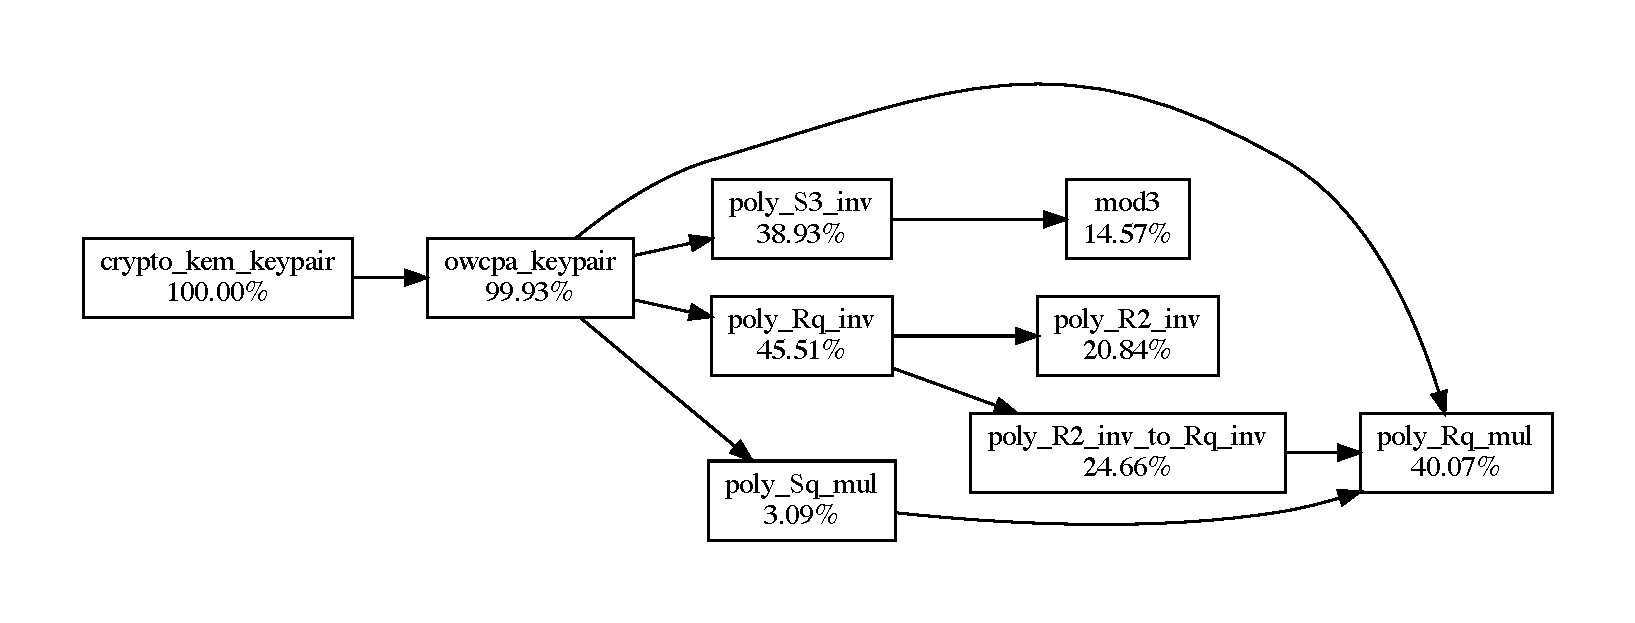
\includegraphics[scale=0.5]{chapters/results/hot-paths/ntru/crypto_kem_keypair.pdf}
    \caption{Relative instruction count of \gls{ntru}'s \textit{crypto\_kem\_keypair}}
    \label{figure:result:hot-paths:ntru:crypto_kem_keypair}
\end{figure}

Figure \ref{figure:result:hot-paths:ntru:crypto_kem_enc} describes the encapsulation API function. The key is generated using random bytes which are fed through 256-bit \gls{aes} in its Electronic Code Book (ECB) configuration to produce uniformly random bytes. Again, we see a significant percentage of the instructions spent in the polynomial library - in \textit{poly\_Rq\_mul}.

\begin{figure}[H]
    \centering
    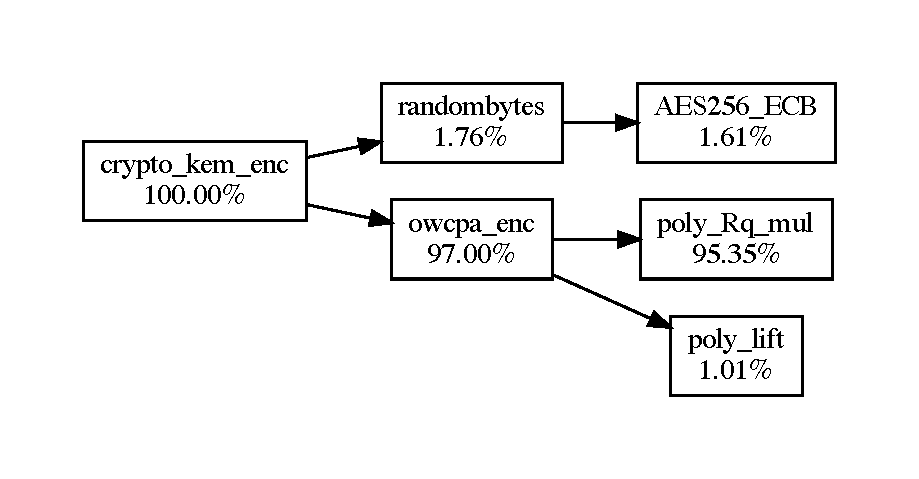
\includegraphics[scale=0.5]{chapters/results/hot-paths/ntru/crypto_kem_enc.pdf}
    \caption{Relative instruction count of \gls{ntru}'s \textit{crypto\_kem\_keypair}}
    \label{figure:result:hot-paths:ntru:crypto_kem_enc}
\end{figure}

The decryption function of \gls{ntru} is presented in figure \ref{figure:result:hot-paths:ntru:crypto_kem_dec}. Virtually all of the instructions spent decrypting (decapsulating) a key is spent in the \textit{poly\_Rq\_mul} function.

\begin{figure}[H]
    \centering
    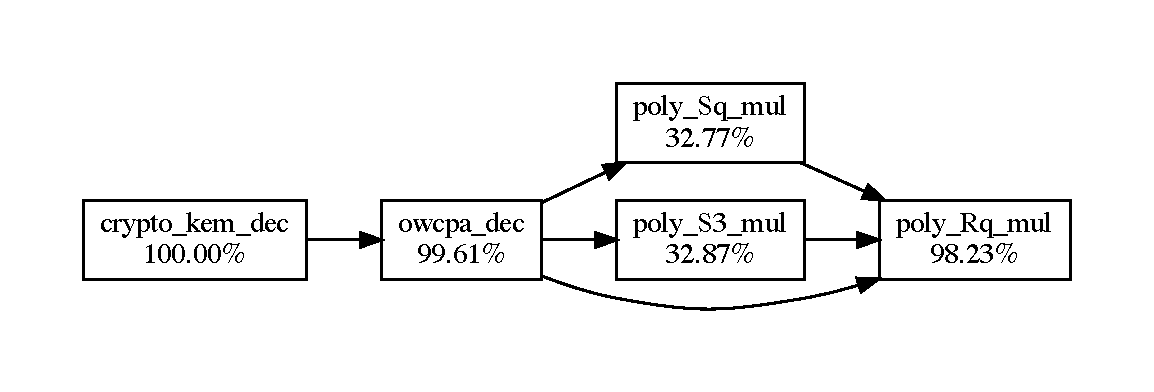
\includegraphics[scale=0.5]{chapters/results/hot-paths/ntru/crypto_kem_dec.pdf}
    \caption{Relative instruction count of \gls{ntru}'s \textit{crypto\_kem\_dec}}
    \label{figure:result:hot-paths:ntru:crypto_kem_dec}
\end{figure}

Looking at the code of \textit{poly\_Rq\_mul} as shown in figure \ref{figure:result:hot-paths:ntru:poly_Rq_mul}, it is evident that the vast majority of instructions are spent on multiplying and adding numbers in loops. The value of \textit{NTRU\_N} corresponds to the parameter set. For \gls{ntru} HRSS 701, the value is 701 and for \gls{ntru} HPS 4096821 the value is 821.

\begin{figure}[H]
    \centering
    \begin{lstlisting}[language=C]
void poly_Rq_mul(poly *r, const poly *a, const poly *b) {
  int k, i;

  for (k = 0; k < NTRU_N; k++) {
    r->coeffs[k] = 0;
    for (i = 1; i < NTRU_N - k; i++) // 10.21%
      r->coeffs[k] += a->coeffs[k + i] * b->coeffs[NTRU_N - i]; // 42.75%
    for (i = 0; i < k + 1; i++) // 8.20%
      r->coeffs[k] += a->coeffs[k - i] * b->coeffs[i]; // 38.79%
  }
}
    \end{lstlisting}
    \caption{Annotated source code of \gls{ntru}'s \textit{poly\_Rq\_mul}}
    \label{figure:result:hot-paths:ntru:poly_Rq_mul}
\end{figure}

To summarize, it is shown that factors such as the speed of \gls{aes} has little to do with the overall performance of the algorithm. Furthermore, it seems as if the polynomial library functions account for the vast majority of instructions spent on key-pair generation, encryption and decryption. The function \textit{poly\_Rq\_mul}, which multiplies two polynomials in $\mathbb{R}^q$, accounts for most of the calculations performed.

\subsection{Classic McEliece}
The \gls{mceliece} reference implementation consists of three API methods - \textit{crypto\_kem\_keypair}, \textit{crypto\_kem\_enc} and \textit{crypto\_kem\_dec} for key-pair generation, encryption (encapsulation) and decryption (decapsulation), respectively\todo{A bit CTRL+C CTRL+V from previous, rewrite?}. These API functions may in turn call several internal functions. We will only present the hot-paths for the \gls{mceliece} 8192128 non-f variant because it can quite accurately represent the hot-paths for all \gls{mceliece} variants.

In figure \ref{figure:result:hot-paths:classic-mceliece:crypto_kem_keypair}, we can see the \textit{crypto\_kem\_keypair} function and its only significant internal function, the \textit{pk\_gen} function that takes up 98.57\% of the execution time. In figure \ref{figure:result:hot-paths:classic-mceliece:pk_gen}, a more in-depth representation of the \textit{pk\_gen} function is presented. In that figure, all of its internal functions are shown. As can be seen, they do not make up much of the accumulated instruction counts. Most of the instructions are inside of the \textit{pk\_gen} function itself.

\begin{figure}[H]
    \centering
    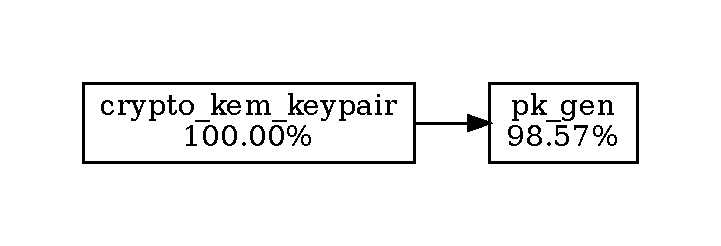
\includegraphics[scale=0.5]{chapters/results/hot-paths/classic-mceliece/8192128/crypto_kem_keypair.pdf}
    \caption{Relative instruction count of \gls{mceliece}'s \textit{crypto\_kem\_keypair}}
    \label{figure:result:hot-paths:classic-mceliece:crypto_kem_keypair}
\end{figure}

\begin{figure}[H]
    \centering
    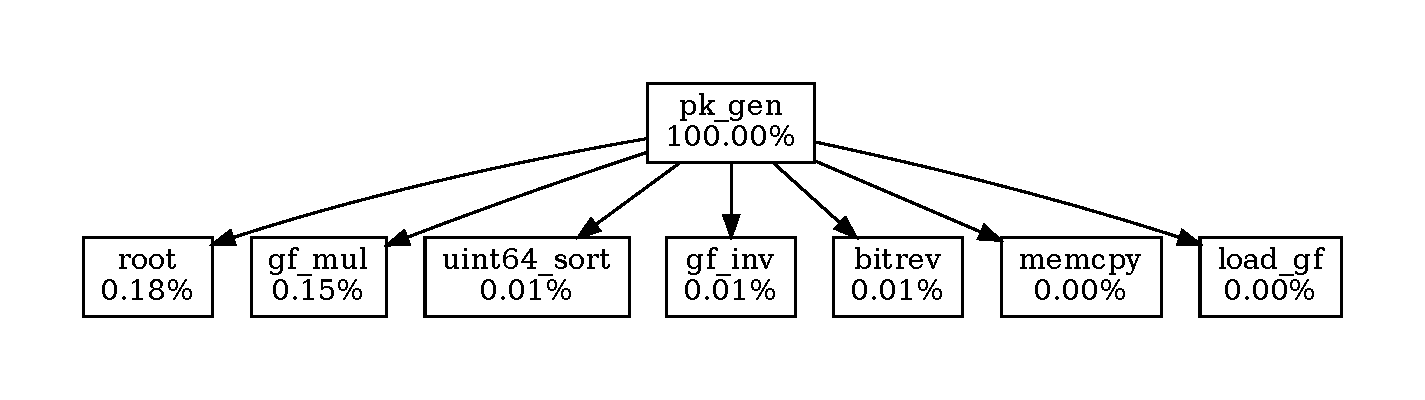
\includegraphics[scale=0.5]{chapters/results/hot-paths/classic-mceliece/8192128/pk_gen.pdf}
    \caption{Relative instruction count of \gls{mceliece}'s \textit{pk\_gen}}
    \label{figure:result:hot-paths:classic-mceliece:pk_gen}
\end{figure}

The encryption function of \gls{mceliece} is presented in figure \ref{figure:result:hot-paths:classic-mceliece:crypto_kem_enc}. Most time is spent in the syndrome function. In figure \ref{figure:result:hot-paths:classic-mceliece:crypto_kem_enc} the decryption function is presented. The majority of the time is spent in the \textit{synd} function.

\begin{figure}[H]
    \centering
    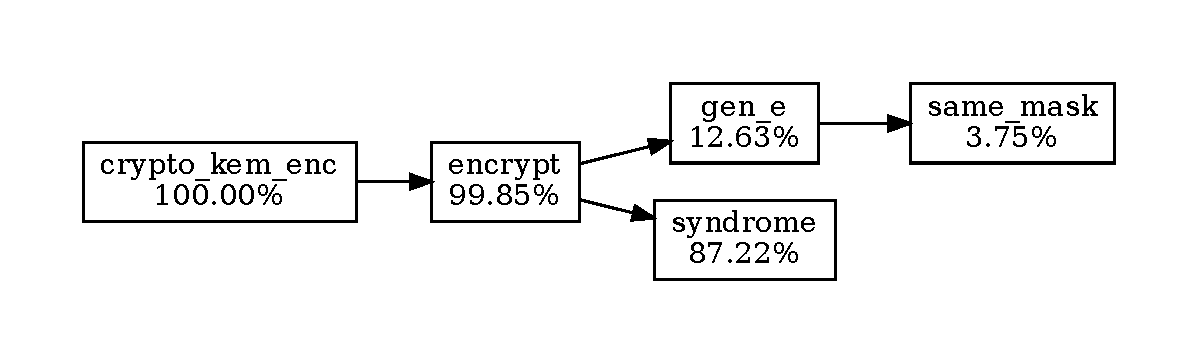
\includegraphics[scale=0.5]{chapters/results/hot-paths/classic-mceliece/8192128/crypto_kem_enc.pdf}
    \caption{Relative instruction count of \gls{mceliece}'s \textit{crypto\_kem\_enc}}
    \label{figure:result:hot-paths:classic-mceliece:crypto_kem_enc}
\end{figure}


\begin{figure}[H]
    \centering
    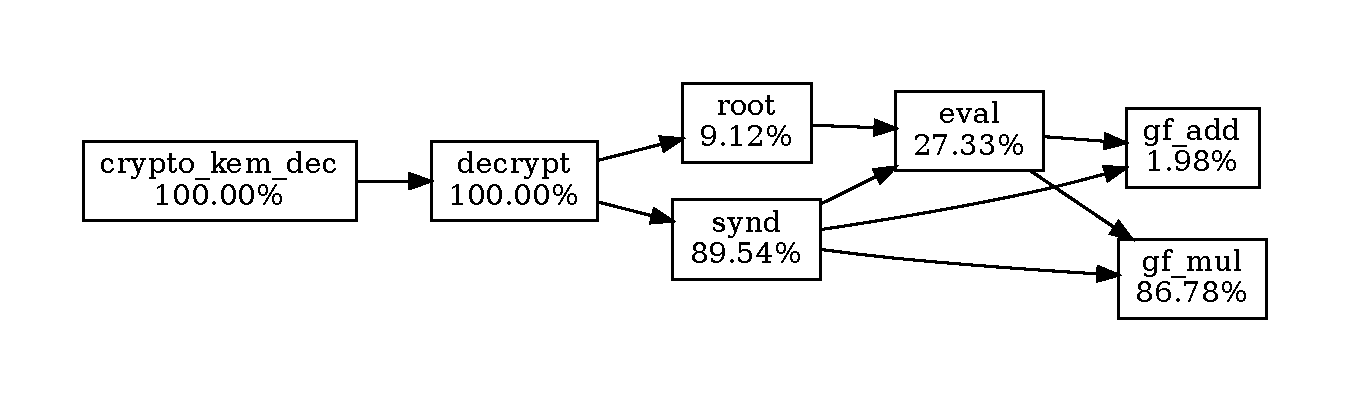
\includegraphics[scale=0.5]{chapters/results/hot-paths/classic-mceliece/8192128/crypto_kem_dec.pdf}
    \caption{Relative instruction count of \gls{mceliece}'s \textit{crypto\_kem\_dec}}
    \label{figure:result:hot-paths:classic-mceliece:crypto_kem_dec}
\end{figure}

\todo[inline]{Var tydliga med hot paths och tid. Exempelvis så lär diagrammet för pk\_gen visa 0\% för vissa funktioner så som root, men om vi ser till hot paths så lär vi se att de kallas flera miljoner gånger. Kanske ha en graf som visar antalet invocations?}

\todo[inline]{Ingen microbenchmark för eval, gf\_mul och gf\_add - de körs så många gånger att overheaden för profiling blev 1000x. McEliece kallar på många många tusen funktioner (hundra tusen, uppemot miljoner?) - det i sig bör ge mer overhead. }

\section{The Performance of Post-Quantum Key Exchange Mechanisms}

This section presents the results of the experiment as outlined in section \ref{section:method:experiment}. It further discusses the performance of \gls{post-quantum} \glspl{kem} and how they may differ on various architectures and hardware.

\subsection{Heap Usage}

As outlined in the method, section \ref{section:method:experiment:phase1:measurements}, we measured the heap usage of the algorithms by monitoring heap allocation and deallocation methods such as malloc using heaptrack. We found that the heap allocation did not change across environments nor between the analyzed optimizations except for some few. As for the implementations, this is rather unsurprising as changing how the allocations worked would alter the behavior of the code. As we found that the heap behavior of the algorithms were consistent throughout our test, we will for the rest of this section not refer to any specific environment or optimization used for the algorithms unless otherwise noted. When talking about allocation, we will refer to the peak allocation - that is, the maximum allocated bytes recorded during a function's lifetime. Our measurements did not capture the peak heap allocation during a benchmark as it would include memory allocations introduced by our tooling. The heap usage metrics do not reflect total memory usage as memory in the form of parameters passed to the algorithms or memory that's part of the stack is not included.

At one point, the \gls{ntru} implementations allocated $264$ bytes generating a keypair. These bytes were allocated by OpenSSL to initialize the library's envelope suite of functions. In context, this is done as the \gls{ntru} implementation uses OpenSSL's \gls{aes} ECB implementation to generate uniform pseduo-random bytes. The invocation of the \gls{aes} function itself resulted in $208$ bytes being allocated by the OpenSSL \gls{aes} ECB implementation. Beyond these bytes, the \gls{ntru} implementation did not require any additional heap allocation during its runtime.

Just like the \gls{ntru} implementations, the \gls{mceliece} implementations make use of OpenSSL to create uniform pseudo-random bytes. As such, the same $264$ bytes are allocated to initialize OpenSSL's envelope suite of functions, as well as the $208$ bytes to actually encrypt random data to produce a uniformly distributed series of bytes. No further allocations were found to be made.

The \gls{ecdhe} and \gls{dhe} implementations are based entirely on functions made available via the OpenSSL library. All of the implementations had an increase in the number of allocations made when compared to \gls{ntru} and \gls{mceliece}. The \gls{dhe} implementation when run in the IBM Community Cloud environment saw an allocation of $16960$ bytes during keypair generation made from a function to calculate the constant-time modulo exponentiation on an arbitrary large number. All other environments allocated $9024$ bytes for the same invocation. Furthermore, the keypair generation saw the allocation of a further $1024$ bytes in the IBM Community Cloud environment seemingly related to the same modulo operation.
The operation of dividing an integer was found to correlate to an additional $536$ bytes in the Cloud Provider 1 environment and $528$ bytes in all of the other environments. The environments saw an additional $1432$ bytes corresponding to the handling of arbitrary large numbers whilst generating a keypair. Fetching random data raised the allocation with $632$ bytes in all environments. There were further allocations made, all of which are summarized in Table \ref{table:results:memory:dhe-heap}. In the table, the peak heap usage of each function of the implementation has been summed up to produce a sum of peaks. This value does not correspond to the peak heap usage of the algorithm as a whole. The \gls{ecdhe} implementation behaved much like the \gls{dhe}, with the peaks differing between some environments. The implementation too worked with OpenSSL's arbitrary numbers and as such had several of the same allocations as the \gls{dhe} implementations. The peaks are presented in Table \ref{table:results:memory:ecdhe-heap}.

\begin{table}
    \centering
    \small
    \caption{Heap Allocation in Bytes for \gls{dhe}}
    \label{table:results:memory:dhe-heap}
    \begin{tabularx}{\linewidth}{X c c c}
        \toprule
        \thead{Environment} & \thead{OpenSSL Version} & \multicolumn{2}{c}{\thead{Sum of Peaks}}\\
        & & \thead{Keypair} & \thead{Exchange} \\
        \midrule
        IBM Community Cloud & 1.1.1g FIPS & 42800 & 39908 \\
        Cloud Provider 1 & 1.1.1 & 14156 & 11934 \\
        Cloud Provider 2 & 1.1.1f & 14040 & 11762\\
        Modern Workstation & 1.1.1f & 14040 & 11762 \\
        Modern Laptop & 1.1.1f & 14040 & 11762 \\
        Old Mid-Range Laptop & 1.1.1f & 14040 & 11762\\
        Old Low-Range Laptop & 1.1.1f & 14040 & 11762\\
        \bottomrule
    \end{tabularx}
\end{table}
\todo{Does not correctly reflect the actual usage? Zero is most likely wrong as the exchange function creates a key. Furthermore, the values currently reflect crypto\_kem\_keypair and crypto\_kem\_exchange, not perform\_keypair and perform\_exchange}

\begin{table}
    \centering
    \small
    \caption{Heap Allocation in Bytes for \gls{ecdhe}}
    \label{table:results:memory:ecdhe-heap}
    \begin{tabularx}{\linewidth}{X c c c c}
        \toprule
        \thead{Environment} & \thead{Curve} & \thead{OpenSSL Version} & \multicolumn{2}{c}{\thead{Sum of Peaks}}\\
        & & & \thead{Keypair} & \thead{Exchange} \\
        \midrule
        IBM Community Cloud & P-256 & 1.1.1g FIPS & 12184 & 0 \\
        IBM Community Cloud & 25519 & 1.1.1g FIPS & 4524 & 1024 \\

        Cloud Provider 1 & P-256 & 1.1.1 & 9220 & 0 \\
        Cloud Provider 1 & 25519 & 1.1.1 & 8380 & 0 \\

        Cloud Provider 2 & P-256 & 1.1.1f & 4884 & 1872 \\
        Cloud Provider 2 & 25519 & 1.1.1f & 2556 & 512\\

        Modern Workstation & P-256 & 1.1.1f & 4884 & 1872 \\
        Modern Workstation & 25519 & 1.1.1f & 2556 & 512 \\
        
        Modern Laptop & P-256 & 1.1.1f & 4884 & 1872 \\
        Modern Laptop & 25519 & 1.1.1f & 2556 & 512 \\
        
        Old Mid-Range Laptop & P-256 & 1.1.1f & 4884 & 1872\\
        Old Mid-Range Laptop & 25519 & 1.1.1f & 2556 & 512\\
        
        Old Low-Range Laptop & P-256 & 1.1.1f & 4884 & 1872\\
        Old Low-Range Laptop & 25519 & 1.1.1f & 2556 & 512\\
        \bottomrule
    \end{tabularx}
\end{table}
\todo[inline]{Does not correctly reflect the actual usage? Zero is most likely wrong as the exchange function creates a key. Furthermore, the values currently reflect crypto\_kem\_keypair and crypto\_kem\_exchange, not perform\_keypair and perform\_exchange

Is this all due to OpenSSL allocating and handling its own memory? Easy to blame them...
}

\subsection{Stack Usage}

In terms of stack usage, the results vary between the implementations, compilers and features. For instance, the polynomial math function poly\_Rq\_mul in \gls{ntru}, which was identified as constituting most of the time spent in the algorithm, varies between taking up $70499$ and $188$ bytes. In all environments, the HPS 4096821 AVX2 variant takes up $70499$ bytes. This does not change between compilers or optimization flags, which could be due to the fact that the implementation is written in assembly - leaving little room for the compiler to alter the behavior. The same goes for the HRSS 701 variant of \gls{ntru} - the size is consistently 55317 bytes across environments and optimization flags. The lowest sizes are found when the reference implementation is compiled with optimization. The sizes are presented in Table \ref{table:results:memory:ntru-stack}. Although the optimization flags used were not chosen for improving the size of the binary, the size of the function has been lowered in all cases. Although the same version of GCC was used for several environments, the results differed between $188$ and $192$ bytes. Clang continually produced larger regions than GCC. Furthermore, more recent versions of the compilers seem to have produced smaller sizes.

\begin{table}
    \small
    \centering
    \caption{Stack Size of poly\_Rq\_mul in Bytes for the Optimized Reference Implementation}
    \label{table:results:memory:ntru-stack}
    \begin{tabularx}{\linewidth}{X c c c c}
        \toprule
        \thead{Environment} & \thead{Compiler} & \thead{Compiler Version} & \thead{Optimized Size} & \thead{Reference Size}\\
        \midrule
        Cloud Provider 1 & clang & 6.0.0 & 702 & - \\
        IBM Community Cloud & clang & 10.0.1 & 522 & - \\
        Cloud Provider 2 & clang & 10.0.0 & 380 & - \\
        Modern Laptop & clang & 10.0.0 & 380 & - \\
        Modern Workstation & clang & 10.0.0 & 380 & - \\
        Modern Laptop & clang & 10.0.0 & 380 & - \\
        Old Low-Range Laptop & clang & 10.0.0 & 300 & - \\
        Old Mid-Range Laptop & clang & 10.0.0 & 300 & - \\
    
        IBM Community Cloud & gcc & 8.3.1 & 242 & 382 \\
        Old Low-Range Laptop & gcc & 9.3.0 & 196 & 255 \\
        Old Mid-Range Laptop & gcc & 9.3.0 & 196 & 255 \\
        Cloud Provider 1 & gcc & 7.5.0 & 192 & 253\\
        Cloud Provider 2 & gcc & 9.3.0 & 188 & 255\\
        Modern Laptop & gcc & 9.3.0 & 188 & 255\\
        Modern Workstation & gcc & 9.3.0 & 188 & 255\\
        \bottomrule
    \end{tabularx}
\end{table}

The same correlation between optimization flags and compiler versions could not be found in the case of \gls{mceliece} and pk\_gen. In that case, the largest recorded size was found in IBM Community Cloud's optimized reference implementation with $22858$ bytes. The optimized AVX2 implementation of the Modern Workstation and Modern Laptop came second with $22123$ bytes. Lastly, the smallest size recorded was found in the optimized reference implementation of Old Mid-Range Laptop and Old Low-Range Laptop at $2026$ bytes.

As for other functions of the \glspl{kem}, the data is too massive to comprehensively refer to here. There are, however, tables in the appendix for average sizes as compared to the reference implementation compiled with GCC. In Table \ref{table:result:ntru-average-stack-increase-cloud}, for example, one may see that Clang seems to produce smaller binaries. Furthermore, the optimized AVX2 builds result in the largest binaries - with symbols taking 8-10 times the size of the reference implementation.

\todo[inline]{Discuss stack usage of ECDHE, DHE?}

\subsection{Parameter Sizes}

The measurements presented up until this point have been related to either the runtime behavior of the algorithms, or the static requirements they place on the environment in the form of stack usage. These measurements have not included the parameters fed to the algorithms - which could affect real-world applications. The remaining part of this section will present data gathered from the various implementations.

The \glspl{kem} tested conform to the same API. Their signatures are presented in figure \ref{figure:result:memory:kem-api}. The function crypto\_kem\_keypair, which generates a keypair takes in a public key and a secret key. The encapsulation function, crypto\_kem\_enc, takes in a ciphertext buffer, a key buffer and the public key of a peer. Lastly, the decapsulation function, crypto\_kem\_dec takes in a key buffer, the ciphertext as received from a peer and the secret key. The sizes of these parameters differ between algorithms and implementations - but is not changed depending on the environment or optimizations. Table \ref{table:results:memory:kem-parameter-sizes} shows the sizes of the parameters in bytes. The sizes do not differ between the semi-systematic (f) variants of \gls{mceliece}. Therefore only two variants of \gls{mceliece} are presented.

\begin{figure}
    \centering
    \begin{lstlisting}[language=C]
int crypto_kem_keypair(unsigned char *public_key, unsigned char *private_key);
int crypto_kem_enc(unsigned char *ciphertext, unsigned char *key, const unsigned char *public_key);
int crypto_kem_dec(unsigned char *key, const unsigned char *ciphertext, const unsigned char *private_key);
    \end{lstlisting}
    \caption{The API of the \gls{kem} Implementations}
    \label{figure:result:memory:kem-api}
\end{figure}

\begin{table}
    \centering
    \small
    \caption{Parameter Sizes in Bytes of the \glspl{kem} Under Test}
    \label{table:results:memory:kem-parameter-sizes}
    \begin{tabularx}{\linewidth}{X c c c c c}
        \toprule
        \thead{Algorithm} & \thead{Parameters} & \thead{public\_key} & \thead{private\_key} & \thead{ciphertext} & \thead{key}\\
        \midrule
        \gls{mceliece} & 8192128(f) & 1357824 & 14120 & 240 & 32 \\
        \gls{mceliece} & 6960119(f) & 1047319 & 13948 & 226 & 32 \\
        \gls{ntru} & HRSS 701 & 1138 & 1450 & 1138 & 32 \\
        \gls{ntru} & HPS 4096821 & 1230 & 1590 & 1230 & 32 \\
        \bottomrule
    \end{tabularx}
\end{table}

The APIs are similar, but not the same for the \gls{kex} implementations. That is due to \gls{dh} requiring the so called Diffie-Hellman Parameters $p$ and $g$. The APIs are shown in figure \ref{figure:results:memory:kex-api}. As with the \gls{kem} implementations, the \gls{kex} implementations use two buffers for a public and a private key when generating a keypair. The \gls{dh} implementation also requires the previously mentioned domain parameters $p$ and $g$ - both buffers of bytes containing the respective parameter. The crypto\_dh\_enc functions further use a key buffer. There is no analogous ciphertext as the \glspl{kex} are fundamentally different from the \glspl{kem} as covered in \ref{section:background:diffie-hellman}. The sizes of the parameters are presented in Table \ref{table:results:memory:kex-parameter-sizes}.

\begin{figure}
    \centering
    \begin{lstlisting}[language=C]
// Diffie-Hellman
int crypto_dh_keypair(unsigned char *public_key, unsigned char *private_key, unsigned char *p, unsigned char *g);

// Diffie-Hellman
int crypto_dh_enc(unsigned char *key, const unsigned char *private_key, const unsigned char *public_key, unsigned char *p, unsigned char *g);

// Elliptic-Curve Diffie-Hellman
int crypto_dh_keypair(unsigned char *public_key, unsigned char *private_key);

// Elliptic-Curve Diffie-Hellman
int crypto_dh_enc(unsigned char *key, const unsigned char *private_key, const unsigned char *public_key);
    \end{lstlisting}
    \caption{The API of the \gls{kex} Implementations}
    \label{figure:results:memory:kex-api}
\end{figure}

\begin{table}
    \centering
    \small
    \caption{Parameter Sizes in Bytes of the \glspl{kex} Under Test}
    \label{table:results:memory:kex-parameter-sizes}
    \begin{tabularx}{\linewidth}{X c c c c c c}
        \toprule
        \thead{Algorithm} & \thead{Parameters} & \thead{public\_key} & \thead{private\_key} & \thead{$p$} & \thead{$g$} & \thead{key}\\
        \midrule
        \gls{dh} & 2048    &255 & 255 & 256  & 1 & 32 \\
        \gls{ecdh} & P-256 & 65 & 32 & - & - & 32 \\
        \gls{ecdh} & 25519 & 32 & 32 & - & - & 32 \\
        \bottomrule
    \end{tabularx}
\end{table}

\subsection{Sequential Performance}

The performance of the algorithms in a single run was analyzed by performing a thousand sequential runs in series, for each algorithm under test at two different occasions. The complete method is outlined in section \ref{section:method:experiment:phase1}.

As covered in section \ref{section:background:mceliece}, \gls{mceliece} supports two forms of keypair-generation algorithms - a systematic form and a semi-systematic form. The systematic forms, such as \gls{mceliece} 8192128 and the semi-systematic forms, such as \gls{mceliece} 8192128f, use different algorithms for generating the keypairs. The authors of the \gls{nist} submission state that these two forms may have different performance characteristics \cite{mceliece2020}. In Table \ref{table:results:sequential-mceliece-6960119-keypair-modern-workstation}, these two forms can be seen with every set of performance improvements tested in the experiment. As can be seen in the table, the reference implementation in its systematic form is remarkably inconsistent, with a standard deviation of $20580.20$ as compared to the $6.91$ of the semi-systematic form. The change in performance characteristics is also visible in the mean, with the semi-systematic form taking about $30\%$ of the time on average as compared to the systematic form. In both cases, the \gls{avx2} implementation has the second largest standard deviation with $302.58$ and $6.91$ for the systematic form and the semi-systematic form, respectively. Despite being a \gls{simd} implementation, \gls{avx2} performs worse than the optimized reference implementation in both forms of the algorithm. The optimized \gls{avx2} implementation, however, outperforms the optimized reference implementation with four to six times the performance. The same results were found to generalize for several environments, as shown in Table \ref{table:results:sequential:mceliece-6960119-keypair} and \ref{table:results:sequential:mceliece-6960119f-keypair}.

\begin{table}
    \centering
    \caption{Duration of \gls{mceliece} 6960119 Keypair Generation On Modern Workstation}
    \label{table:results:sequential-mceliece-6960119-keypair-modern-workstation}
    \begin{tabularx}{\linewidth}{l X c c c c}
        \toprule
        \thead{Compiler} & \thead{Flags} & \thead{Mean} & \thead{Standard\\Deviation} & \multicolumn{2}{c}{\thead{95\% CI}}\\
        & & & & \thead{Lower} & \thead{Upper} \\
        \midrule
        \thead{non-systematic form}\\
                         gcc &                  ref &             21885.78 &             20580.20 &             17376.37 &             26395.19\\
                         gcc &                 avx2 &               562.39 &               302.58 &               549.13 &               575.66\\
                       clang &        ref-optimized &               696.65 &               571.35 &               671.60 &               721.70\\
                         gcc &        ref-optimized &               421.15 &               317.77 &               407.22 &               435.09\\
                         gcc &       avx2-optimized &                72.26 &                38.78 &                70.56 &                73.96\\
                       clang &       avx2-optimized &                70.28 &                38.12 &                68.61 &                71.95\\
    
    \midrule
      \thead{semi-systematic form}\\
                        gcc &                  ref &              6476.15 &                 6.91 &              6475.33 &              6476.97\\
                         gcc &                 avx2 &               315.24 &                 0.96 &               315.19 &               315.28\\
                       clang &        ref-optimized &               230.14 &                 0.74 &               230.11 &               230.18\\
                         gcc &        ref-optimized &               159.12 &                 0.61 &               159.09 &               159.15\\
                         gcc &       avx2-optimized &                40.45 &                 0.84 &                40.42 &                40.49\\
                       clang &       avx2-optimized &                39.93 &                 1.50 &                39.86 &                39.99\\
        \bottomrule
    \end{tabularx}
\end{table}

In all environments but one, we found consistent performance throughout all sequential runs, non-deterministic behavior and outliers aside. The Cloud Provider 2 environment provided inconsistent results throughout the sequential performance benchmarks - across various algorithms and runs. As seen in figure \ref{figure:results:sequential:mceliece-decrpyt-cloud-provider-2}, there are several occasions where the performance shift over time. In the figure, the speedup relative to the reference GCC implementation is used as opposed to the absolute duration of each iteration. Depending on how deterministic the behavior of the algorithms are, as well as how stable the environment is, one could have expected more or less the same performance throughout the test. As the Cloud Provider 2 environment uses two virtual CPU cores, it is not entirely unexpected to find such inconsistent results. The same behavior was not found in any of the environments tested with dedicated hardware, nor the Cloud Provider 1 environment.

\begin{figure}
    \centering
    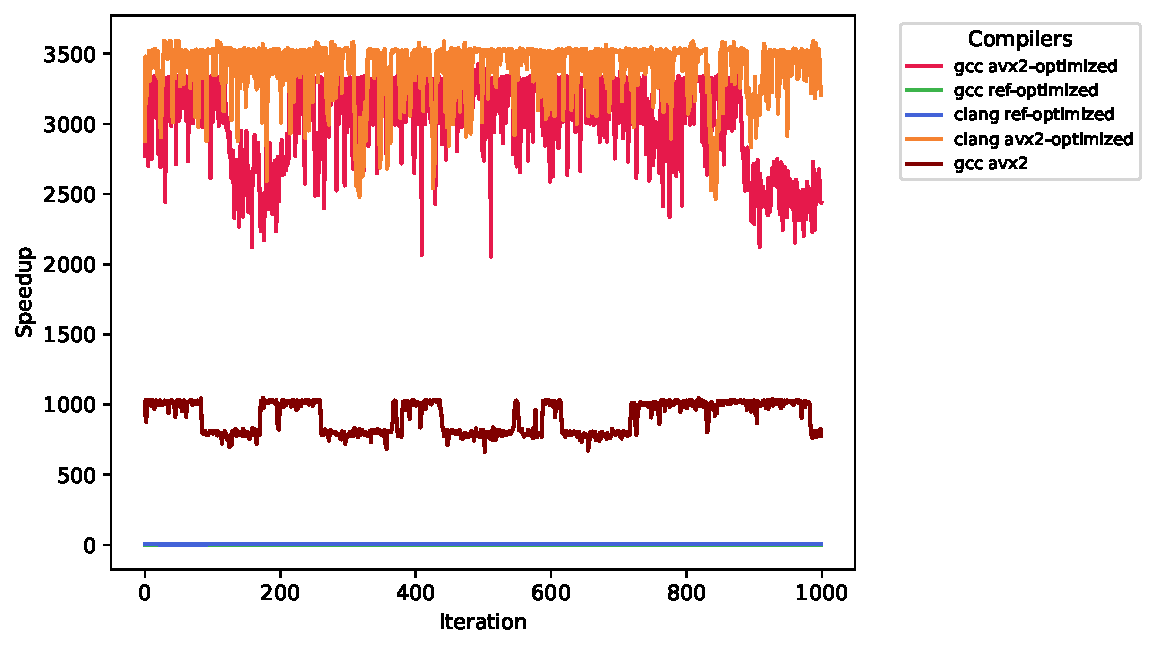
\includegraphics[scale=0.75]{chapters/results/sequential/mceliece_6960119_decrypt_Cloud Provider 2.pdf}
    \caption{The Speedup of \gls{mceliece} 6960119 Over Time. Note that the green and blue lines are coincident}
    \label{figure:results:sequential:mceliece-decrpyt-cloud-provider-2}
\end{figure}

In Table \ref{figure:results:sequential:ntru-hrss701} all of the average durations and speedups for each optimization and environment are shown. In the table, one may see conclusive evidence that the optimized \gls{avx2} implementations perform the best in all environments with support for \gls{avx2}. It is not clear, however, what compiler produces the best performance. In the environments without support for \gls{avx2}, the optimized reference implementation performed the best. Just as with the \gls{avx2} implementations, it's unclear whether or not GCC or Clang produced the best results. It seems as if GCC produces more consistent results, with less variation in the averages. In the Old Low-Range Laptop environment, for example, one may see that Clang requires about two times the duration of the comparable subject compiled with GCC. In other cases, Clang seems to be on par with, or better than, GCC. As the speedup is percentual based on the environment, one may expect them to be similar across environments. That is, the speedup of using \gls{avx2} instead of the reference implementation, should in theory be similar on both the Modern Workstation and Modern Laptop, for example. In practice we found this to not be true. Although similar, the \gls{avx2} implementation compiled and optimized by Clang on the Modern Workstation has an additional 78 times speedup when compared to the Modern Laptop. On the other hand, the Old Mid-Range Laptop and the Old Low-Range Laptop perform near identically in terms of speedup.

\begin{table}[H]
    \centering
    \footnotesize
    \caption{Sequential Duration and Speedup of \gls{ntru} HRSS 701}
    \label{figure:results:sequential:ntru-hrss701}
    \begin{tabularx}{\linewidth}{l l c c c c c c}
        \toprule
        \thead{Environment} & \thead{Flags} & \multicolumn{3}{c}{\thead{Average Duration (ms)}} & \multicolumn{3}{c}{\thead{Speedup}}\\
        & & keypair & encrypt & decrypt & keypair & encrypt & decrypt \\
        \midrule
        \multirowcell{8}{Modern\\ Workstation}
          & \textbf{gcc} & & & & & \\
          & ref & 34.373 & 0.910 & 2.660 & 0.0 & 0.0 & 0.0\\
          & ref-optimized & 3.386 & 0.235 & 0.641 & 9.2 & 2.9 & 3.2\\
          & avx2 & 0.240 & 0.029 & 0.037 & 142.2 & 30.8 & 71.1\\
          & avx2-optimized & 0.066 & 0.018 & 0.016 & 517.4 & 49.7 & 167.3\\
          & \textbf{clang} & & & & & \\
          & ref-optimized & 5.786 & 0.206 & 0.563 & 4.9 & 3.4 & 3.7\\
          & avx2-optimized & 0.070 & 0.016 & 0.015 & 491.8 & 54.3 & 181.2\\
          \midrule
          \multirowcell{8}{Modern\\ Laptop}
          & \textbf{gcc} & & & & & \\
          & ref & 41.808 & 1.149 & 3.321 & 0.0 & 0.0 & 0.0\\
          & ref-optimized & 4.202 & 0.278 & 0.816 & 8.9 & 3.1 & 3.1\\
          & avx2 & 0.322 & 0.051 & 0.048 & 128.9 & 21.5 & 67.7\\
          & avx2-optimized & 0.085 & 0.026 & 0.024 & 491.4 & 42.5 & 138.3\\
          & \textbf{clang} & & & & & \\
          & ref-optimized & 7.250 & 0.264 & 0.772 & 4.8 & 3.4 & 3.3\\
          & avx2-optimized & 0.087 & 0.024 & 0.032 & 479.0 & 46.1 & 103.1\\
          \midrule
          \multirowcell{5}{Old\\ Mid-Range\\ Laptop}
          & \textbf{gcc} & & & & & \\
          & ref & 61.040 & 1.579 & 4.584 & 0.0 & 0.0 & 0.0\\
          & ref-optimized & 6.376 & 0.416 & 1.131 & 8.6 & 2.8 & 3.1\\
          & \textbf{clang} & & & & & \\
          & ref-optimized & 12.342 & 0.483 & 1.305 & 3.9 & 2.3 & 2.5\\
          \midrule
          \multirowcell{5}{Old\\ Low-Range\\ Laptop}
          & \textbf{gcc} & & & & & \\
          & ref & 77.043 & 1.952 & 5.667 & 0.0 & 0.0 & 0.0\\
          & ref-optimized & 7.929 & 0.502 & 1.391 & 8.7 & 2.9 & 3.1\\
          & \textbf{clang} & & & & & \\
          & ref-optimized & 15.615 & 0.600 & 1.670 & 3.9 & 2.3 & 2.4\\
          \midrule
          \multirowcell{8}{Cloud\\ Provider\\ 1}
          & \textbf{gcc} & & & & & \\
          & ref & 50.464 & 1.353 & 3.959 & 0.0 & 0.0 & 0.0\\
          & ref-optimized & 5.607 & 0.394 & 1.091 & 8.0 & 2.4 & 2.6\\
          & avx2 & 0.408 & 0.056 & 0.065 & 122.7 & 23.3 & 60.2\\
          & avx2-optimized & 0.114 & 0.027 & 0.028 & 442.4 & 49.8 & 142.7\\
          & \textbf{clang} & & & & & \\
          & ref-optimized & 8.137 & 0.286 & 0.797 & 5.2 & 3.7 & 4.0\\
          & avx2-optimized & 0.108 & 0.031 & 0.029 & 465.6 & 43.1 & 134.6\\
          \midrule
          \multirowcell{8}{Cloud\\ Provider\\ 2}
          & \textbf{gcc} & & & & & \\
          & ref & 59.660 & 1.593 & 4.686 & 0.0 & 0.0 & 0.0\\
          & ref-optimized & 5.778 & 0.404 & 1.106 & 9.3 & 2.9 & 3.2\\
          & avx2 & 0.477 & 0.051 & 0.068 & 124.2 & 30.5 & 68.4\\
          & avx2-optimized & 0.148 & 0.057 & 0.054 & 400.9 & 26.9 & 86.4\\
          & \textbf{clang} & & & & & \\
          & ref-optimized & 10.064 & 0.367 & 0.966 & 4.9 & 3.3 & 3.9\\
          & avx2-optimized & 0.130 & 0.037 & 0.030 & 458.8 & 42.3 & 152.6\\
          \midrule
          \multirowcell{5}{IBM\\ Community\\ Cloud}
          & \textbf{gcc} & & & & & \\
          & ref & 63.455 & 2.105 & 6.066 & 0.0 & 0.0 & 0.0\\
          & ref-optimized & 7.202 & 0.485 & 1.426 & 7.8 & 3.3 & 3.3\\
          & \textbf{clang} & & & & & \\
          & ref-optimized & 8.815 & 0.389 & 1.136 & 6.2 & 4.4 & 4.3\\
        \bottomrule
    \end{tabularx}
\end{table}

By studying the average duration taken by the various subjects in each environment, one may clearly see that \gls{avx2} performs the best when it's available. When \gls{avx2} is not available, the optimized reference implementation performs the best. The results are however indecisive in terms of what compiler performed the best in each environment.

\begin{table}[H]
    \centering
    \small
    \caption{Comparison of CPU Cycles of Our and the Submission Authors' Measurements}
    \label{table:results:sequential:nist-vs-ours}
    \begin{tabularx}{\linewidth}{X c r r r r}
        \toprule
        \thead{Algorithm} & \thead{Operation} & \multicolumn{2}{c}{Reference Cycles} & \multicolumn{2}{c}{AVX2 Cycles}\\
        & & \thead{Ours} & \thead{Theirs} & \thead{Ours} & \thead{Theirs}\\
        \midrule
        \multicolumn{4}{l}{\gls{mceliece}}\\
        mceliece6960119 & keypair & 2063786004 & \multicolumn{1}{c}{-} & 380284953 & 438217685\\
        mceliece6960119f & keypair & 801046672 & \multicolumn{1}{c}{-} & 207228427 & 246508730\\
        mceliece8192128 & keypair & 2227969526 & \multicolumn{1}{c}{-} & 453667430 & 514489441\\
        mceliece8192128f & keypair & 835007190 & \multicolumn{1}{c}{-} & 275660079 & 316202817\\
        
        mceliece6960119(f) & encrypt & 41429828 & \multicolumn{1}{c}{-} & 205954 & 161224\\
        mceliece8192128(f) & encrypt & 40992651 & \multicolumn{1}{c}{-} & 238652 & 178093\\
        
        mceliece6960119(f) & decrypt & 41429828 & \multicolumn{1}{c}{-} & 205954 & 301480\\
        mceliece8192128(f) & decrypt & 40992651 & \multicolumn{1}{c}{-} & 238652 & 326531\\
        \midrule
        \multicolumn{4}{l}{\gls{ntru}}\\
        ntruhps4096821 & keypair & 22392736 & 22511180 & 688900 & 431667\\
        ntruhrss701 & keypair & 16893273 & 16487419 & 320425 & 340823\\
        
        ntruhps4096821 & encrypt & 6782969 & 1566922 & 297125 & 98809\\
        ntruhrss701 & encrypt & 4552302 & 1069326 & 88768 & 50441\\
        
        ntruhps4096821 & decrypt & 18128147 & 4237744 & 104332 & 75384\\
        ntruhrss701 & decrypt & 13511286 & 3113303 & 190756 & 62267\\
        \bottomrule
    \end{tabularx}
\end{table}
\todo{Comment on table, mention that it's Modern Workstation}
% mceliece Ours: ref-optimized modern workstation, theirs Intel  Xeon ref -O3 etc...
% ntru: ours ref-optimized modern workstation, theirs intel i 3-6000? etc...
% ntru ours: avx2-optimized modern ... theris i7-4770K (Haswell)
% supercop 1% av ntruhps4096821, 60% av ntruhrss701 wtf?
% amd64; CoffeeLake (906ea); 2017 Intel Core i7-8700; 6 x 3200MHz; bitvise, supercop-20190910
% https://bench.cr.yp.to/results-kem.html
% NTRU stated that their results were to be presented on the same page, but they were not

\subsection{Throughput Performance}

As outlined in section \ref{section:method:experiment:phase2}, the throughput of the algorithms in each environment under test was evaluated for a series of parallelism configurations. The initial plan was to use the best-performing implementation of each algorithm for each environment, as identified by the sequential benchmarks. The results from the sequential benchmark previously presented were not conclusive and we therefore ended up running the parallel benchmarks on both GCC and Clang builds of the best-performing variant.

The throughput of the \gls{dhe} implementation was found to consistently slow down after the number of threads surpass the number of physical cores multiplied with the degree of \gls{smt}. In figure \ref{figure:results:throughput:dh-old-mid-range-laptop}, the throughput of the Old Mid-Range Laptop can be seen. Old Mid-Range Laptop, a dual core machine with four threads, levels off at the four threads mark. As mentioned previously in section \ref{table:method:experiment:phase1:implementation-configurations}, two variants of \gls{dhe} were tested - one compiled and optimized by GCC, the other by Clang - both of which are presented in the aforementioned figure. The performance difference between the two compilers seem to be negligible, which one may expect as the OpenSSL library used to provide the implementation with virtually all of its functionality is dynamically linked. That means that it is not recompiled nor optimized by the compiler used to compile the program. The same leveling found in Old Mid-Range Laptop was also identified in all of the other environments tested.

\begin{figure}
    \centering
    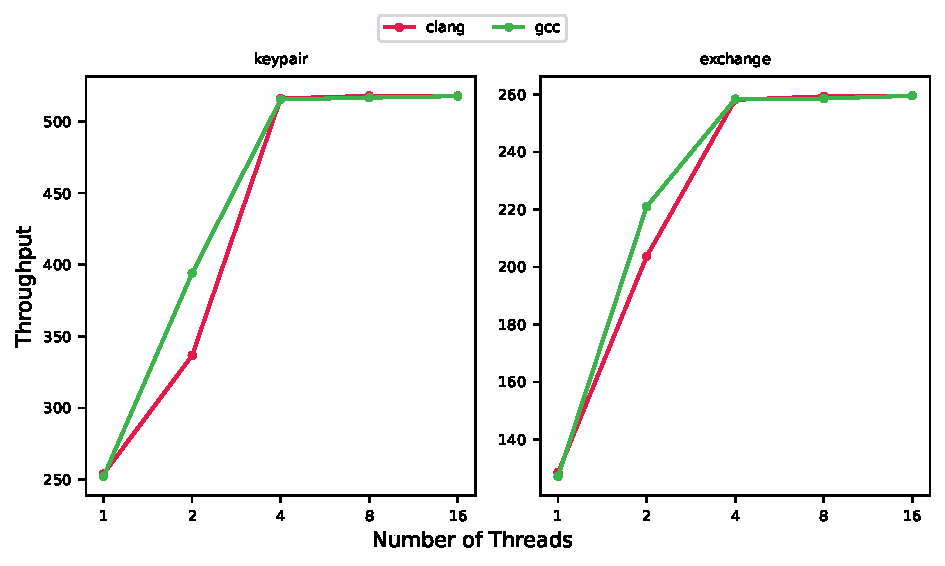
\includegraphics[scale=0.75]{chapters/results/throughput/Old Mid-Range Laptop_dh.pdf}
    \caption{Throughput of \gls{dhe} on Old Mid-Range Laptop for Various Thread Counts}
    \label{figure:results:throughput:dh-old-mid-range-laptop}
\end{figure}

The \gls{ecdhe} implementation was found to be drastically more performant than the \gls{dhe} implementation, with a speedup ranging between 5 to 350 times the throughput. The highest increase in performance was found in the IBM Community Cloud environment, seen in figure \ref{figure:results:throughput:ecdh-ibm-community-cloud}. The throughput, drastically dropped when tested on four or more threads. The peak at two threads coincides with the number of available threads\footnote{It is unknown whether or not the cores are physical cores, logical cores or virtual cores} of the environment. What's more is a 30\% drop in throughput in the exchange phase of the \gls{x25519} implementation compiled and optimized using GCC. The drop was consistent through both of the runs of the complete benchmark at two completely different occasions\todo{analyze further?}. It was found that during the \gls{x25519} run on four threads, two of the threads consistently performed half of the throughput of the other two.

\begin{figure}
    \centering
    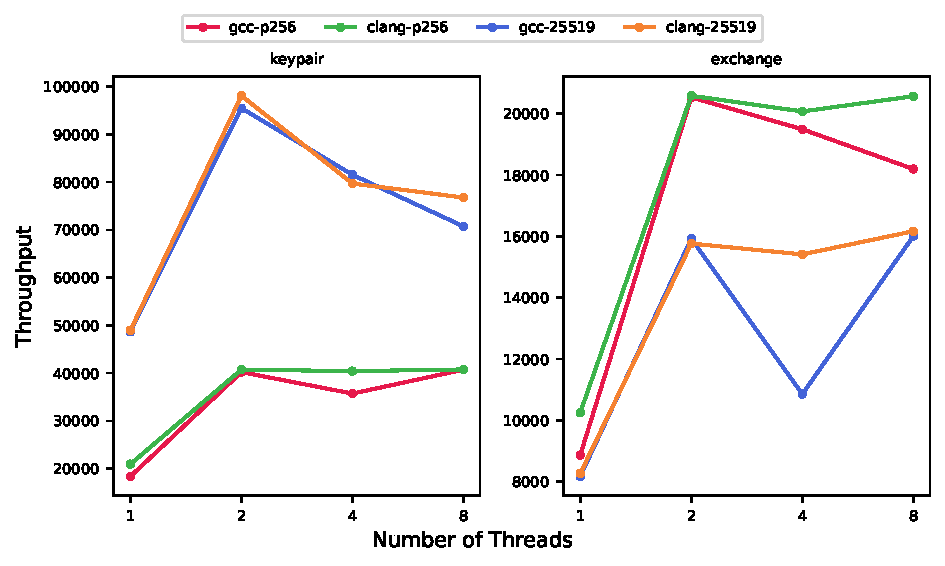
\includegraphics[scale=0.75]{chapters/results/throughput/IBM Community Cloud_ecdh.pdf}
    \caption{Throughput of \gls{ecdhe} on IBM Community Cloud for Various Thread Counts}
    \label{figure:results:throughput:ecdh-ibm-community-cloud}
\end{figure}

In Table \ref{table:results:throughput:ecdh-25519}\todo{explain table}, the throughput for each environment is shown for the \gls{x25519} keypair generation. As can be seen, the IBM Community Cloud environment outperforms all of the other environments when using one or two threads. The mainframe and cloud hardware tested saw a decrease in throughput at one point or another, whilst the consumer hardware continually performed better with more threads for all the thread counts tested\todo{explain table - what optimizations were used, what are the values?}.

    \begin{table}[H]
        \centering
        \small
        \caption{Parallel Throughput Runs for X25519 Keypair Generation}
        \label{table:results:throughput:ecdh-25519}
        \begin{tabularx}{\linewidth}{X c c c c c c c c}
            \toprule
            \thead{Environment} & \thead{Compiler} & \multicolumn{7}{c}{\thead{Threads}}\\
            & & 1 & 2 & 4 & 8 & 16 & 32 & 64 \\
            \midrule
\multirowcell{4}{Cloud\\ Provider\\ 1} & 
\multirow{2}{*}{gcc} & 20066 & 28639 & 41075 & 39385 & 43578\\
 & & 1.0 & 1.43 & 2.05 & 1.96 & 2.17\\
\cmidrule[0.05em](){3-9} & 
\multirow{2}{*}{clang} & 22183 & 28580 & 45468 & 42508 & 45103\\
 & & 1.11 & 1.42 & 2.27 & 2.12 & 2.25\\
            \midrule
\multirowcell{4}{Cloud\\ Provider\\ 2} & 
\multirow{2}{*}{gcc} & 18784 & 35641 & 34956 & 35292\\
 & & 1.0 & 1.90 & 1.86 & 1.88\\
\cmidrule[0.05em](){3-9} & 
\multirow{2}{*}{clang} & 15818 & 35574 & 31504 & 36365\\
 & & 0.84 & 1.89 & 1.68 & 1.94\\
            \midrule
\multirowcell{4}{IBM\\ Community\\ Cloud} & 
\multirow{2}{*}{gcc} & 48666 & 95482 & 81536 & 70727\\
 & & 1.0 & 1.96 & 1.68 & 1.45\\
\cmidrule[0.05em](){3-9} & 
\multirow{2}{*}{clang} & 48960 & 98079 & 79706 & 76773\\
 & & 1.01 & 2.02 & 1.64 & 1.58\\
            \midrule
\multirowcell{4}{Modern\\ Laptop} & 
\multirow{2}{*}{gcc} & 10654 & 22234 & 42188 & 65254 & 68590 & 76830\\
 & & 1.0 & 2.09 & 3.96 & 6.12 & 6.44 & 7.21\\
\cmidrule[0.05em](){3-9} & 
\multirow{2}{*}{clang} & 10605 & 20794 & 41605 & 63372 & 68244 & 77024\\
 & & 1.00 & 1.95 & 3.91 & 5.95 & 6.41 & 7.23\\
            \midrule
\multirowcell{4}{Modern\\ Workstation} & 
\multirow{2}{*}{gcc} & 13458 & 26474 & 51051 & 140658 & 186775 & 204705 & 235189\\
 & & 1.0 & 1.97 & 3.79 & 10.45 & 13.88 & 15.21 & 17.48\\
\cmidrule[0.05em](){3-9} & 
\multirow{2}{*}{clang} & 12728 & 26607 & 51969 & 143312 & 191370 & 205084 & 233812\\
 & & 0.95 & 1.98 & 3.86 & 10.65 & 14.22 & 15.24 & 17.37\\
            \midrule
\multirowcell{4}{Old\\ Low-Range\\ Laptop} & 
\multirow{2}{*}{gcc} & 8880 & 17512 & 24091 & 24448 & 26801\\
 & & 1.0 & 1.97 & 2.71 & 2.75 & 3.02\\
\cmidrule[0.05em](){3-9} & 
\multirow{2}{*}{clang} & 7758 & 19524 & 23932 & 26041 & 26870\\
 & & 0.87 & 2.20 & 2.70 & 2.93 & 3.03\\
            \midrule
\multirowcell{4}{Old\\ Mid-Range\\ Laptop} & 
\multirow{2}{*}{gcc} & 11238 & 20977 & 28151 & 30188 & 31114\\
 & & 1.0 & 1.87 & 2.50 & 2.69 & 2.77\\
\cmidrule[0.05em](){3-9} & 
\multirow{2}{*}{clang} & 10295 & 15511 & 28881 & 30570 & 31859\\
 & & 0.92 & 1.38 & 2.57 & 2.72 & 2.83 \\
            \bottomrule
        \end{tabularx}
    \end{table}
    

When looking at the throughput of \gls{mceliece} in environments which do not support \gls{avx2}, such as the IBM Community Cloud presented in figure \ref{figure:results:throughput:mceliece-ibm-community-cloud}, we found that the keypair and decrypt throughput was significantly lower than that of the encrypt stage. The performance of the decrypt stage was roughly $0.1\%$ of the encrypt stage. Furthermore, the parameter set with the largest parameters - \gls{mceliece} 8192128f achieved a higher encryption throughput than the \gls{mceliece} 6960119f variant\todo{not true! It's the other way around!}. There is also a large difference between the encrypt stage of the subjects compiled and optimized using GCC and those using Clang. Lastly, it seems as if the throughput levels off after the number of used threads surpass the number of available threads. As mentioned, the same overall behavior was found in all of the environments using the optimized reference implementation for benchmarking the parallel throughput, such as Old Mid-Range Laptop in figure \ref{figure:results:throughput:mceliece-old-mid-range-laptop}.

\begin{figure}
    \centering
    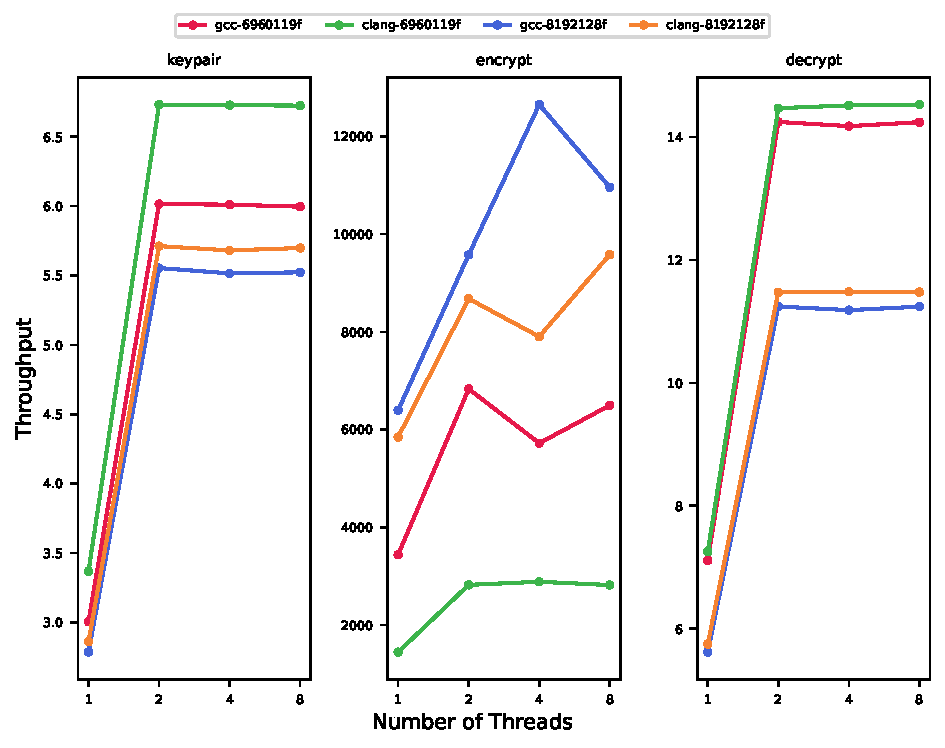
\includegraphics[scale=0.75]{chapters/results/throughput/IBM Community Cloud_mceliece.pdf}
    \caption{Throughput of \gls{mceliece} on IBM Community Cloud for Various Thread Counts}
    \label{figure:results:throughput:mceliece-ibm-community-cloud}
\end{figure} 

\begin{figure}
    \centering
    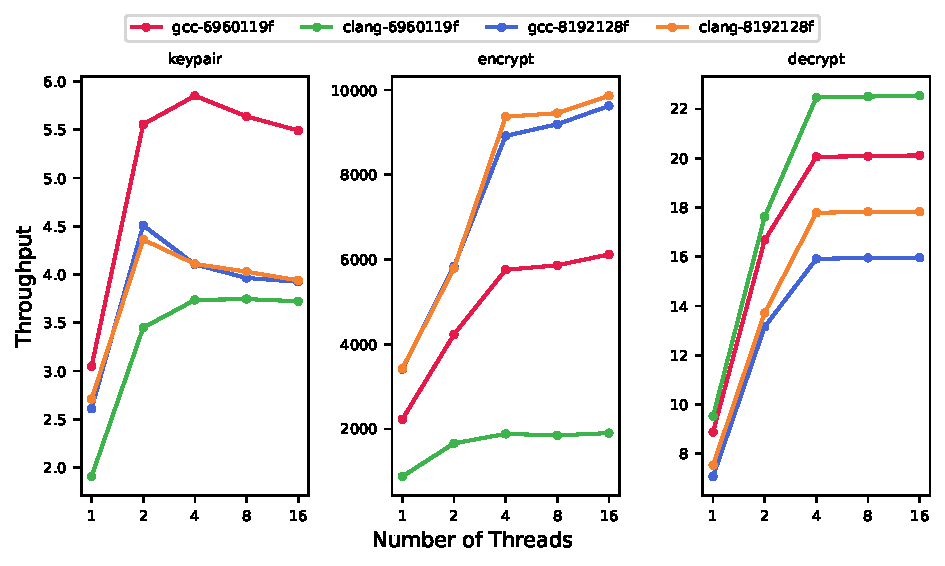
\includegraphics[scale=0.75]{chapters/results/throughput/Old Mid-Range Laptop_mceliece.pdf}
    \caption{Throughput of \gls{mceliece} on Old Mid-Range Laptop for Various Thread Counts}
    \label{figure:results:throughput:mceliece-old-mid-range-laptop}
\end{figure}

When \gls{mceliece} is run in environments with support for \gls{avx2}, such as the Modern Workstation shown in figure \ref{figure:results:throughput:mceliece:modern-workstation}, the results tell a different story. Not only are the compilers much more consistent with one another, but the difference in throughput between the two variants seem to become smaller. It is still clear to see, however, that the smallest parameter size has an overall lower throughput for keypair generation and encryption than the largest parameter size tested\todo{Is this really true? double check!}. The decrypt results seem to show that the smallest parameter size perform the best.

\begin{figure}
    \centering
    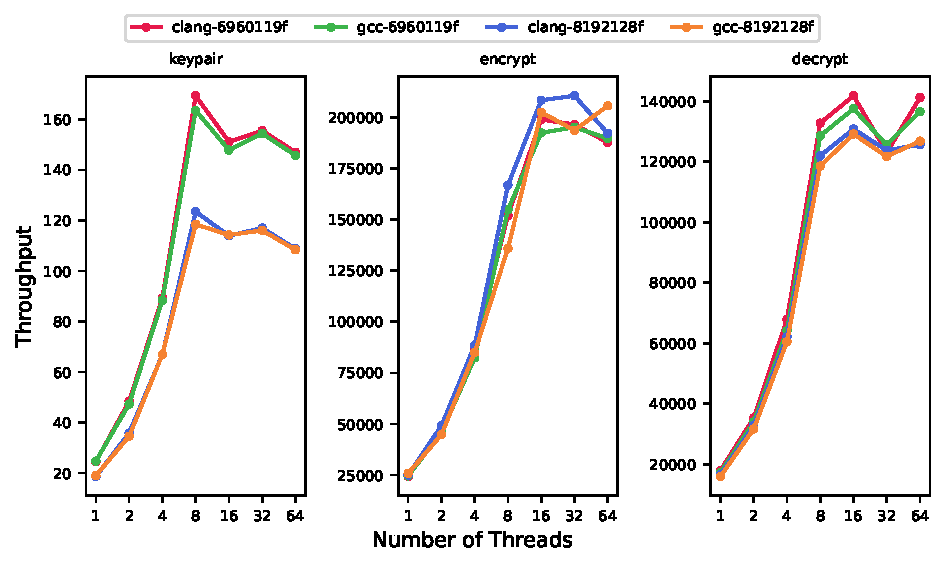
\includegraphics[scale=0.75]{chapters/results/throughput/Modern Workstation_mceliece.pdf}
    \caption{Throughput of \gls{mceliece} on Modern Workstation for Various Thread Counts}
    \label{figure:results:throughput:mceliece-modern-workstation}
\end{figure}

When running \gls{ntru} in parallel to measure throughput, we found that the performance scales well with regards to the number of threads used. In figure \ref{figure:results:throughput:ntru-modern-workstation}, \gls{ntru} HRSS 701 running in the Modern Workstation environment seems to have near-linear scaling for the thread counts tested. The variant also performs considerably better than HPS 4096821 in both the keypair generation stage and the encryption stage. The decrypt stage, however, seems to provide near identical measurements. We found that the same scaling also occurs in the Modern Laptop environment.

\begin{figure}
    \centering
    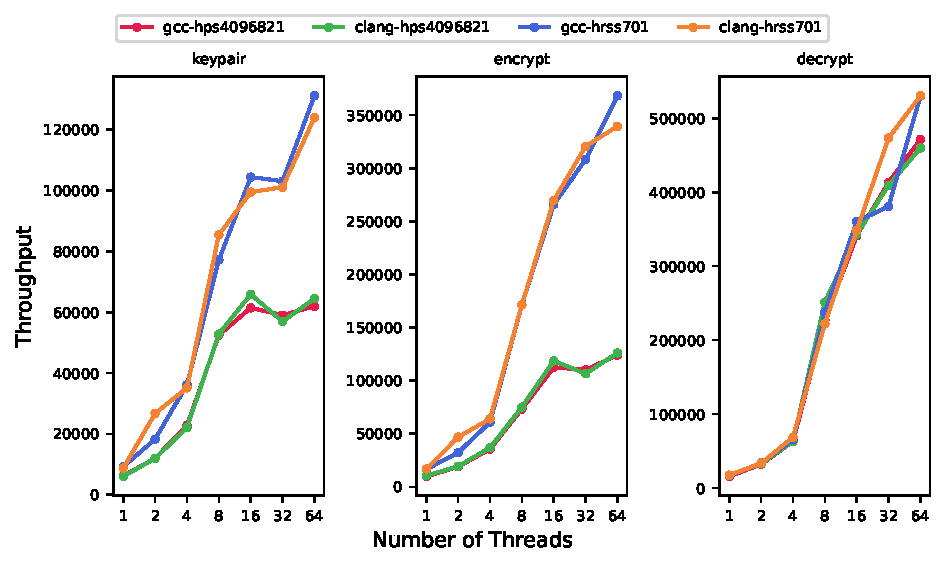
\includegraphics[scale=0.75]{chapters/results/throughput/Modern Workstation_ntru.pdf}
    \caption{Throughput of \gls{ntru} on Modern Workstation for Various Thread Counts}
    \label{figure:results:throughput:ntru-modern-workstation}
\end{figure}

In Table \ref{table:results:throughput:ntru-hrss701-decrypt}, the measurements for various compilers and thread counts are shown for all of the tested environments\todo{explain table}. The best scaling is found in the Modern Workstation environment, followed by the Modern Laptop. Although the tested cloud environments supported \gls{avx2}, they did not see the same performance increase when more threads were used. For all environments except IBM Community Cloud and Cloud Provider 2, GCC seems to produce the highest increase in throughput over the reference implementation compiled with GCC, without performance optimizations.

    \begin{table}[H]
        \centering
        \small
        \caption{Parallel Throughput Runs for ntru hrss701 (decrypt)}
        \label{table:results:throughput:ntru-hrss701-decrypt}
        \begin{tabularx}{\linewidth}{X c c c c c c c c}
            \toprule
            \thead{Environment} & \thead{Compiler} & \multicolumn{7}{c}{\thead{Threads}}\\
            & & 1 & 2 & 4 & 8 & 16 & 32 & 64 \\
            \midrule
\multirowcell{4}{Cloud\\ Provider\\ 1 \footref{avx2-optimized}} & 
\multirow{2}{*}{gcc} & 47064 & 94918 & 94690 & 101730 & 103827\\
 & & 1.0 & 2.02 & 2.01 & 2.16 & 2.21\\
\cmidrule[0.05em](){3-9} & 
\multirow{2}{*}{clang} & 39753 & 71637 & 82847 & 85968 & 85693\\
 & & 0.84 & 1.52 & 1.76 & 1.83 & 1.82\\
            \midrule
\multirowcell{4}{Cloud\\ Provider\\ 2 \footref{avx2-optimized}} & 
\multirow{2}{*}{gcc} & 33224 & 68890 & 74596 & 64194\\
 & & 1.0 & 2.07 & 2.25 & 1.93\\
\cmidrule[0.05em](){3-9} & 
\multirow{2}{*}{clang} & 39840 & 69277 & 62418 & 75534\\
 & & 1.20 & 2.09 & 1.88 & 2.27\\
            \midrule
\multirowcell{4}{IBM\\ Community\\ Cloud \footref{ref-optimized}} & 
\multirow{2}{*}{gcc} & 705 & 1056 & 1373 & 1401\\
 & & 1.0 & 1.50 & 1.95 & 1.99\\
\cmidrule[0.05em](){3-9} & 
\multirow{2}{*}{clang} & 881 & 1772 & 1735 & 1745\\
 & & 1.25 & 2.51 & 2.46 & 2.47\\
            \midrule
\multirowcell{4}{Modern\\ Laptop \footref{avx2-optimized}} & 
\multirow{2}{*}{gcc} & 14694 & 26965 & 94495 & 147789 & 172734 & 176251\\
 & & 1.0 & 1.84 & 6.43 & 10.06 & 11.75 & 11.99\\
\cmidrule[0.05em](){3-9} & 
\multirow{2}{*}{clang} & 13041 & 32001 & 87645 & 104470 & 148045 & 166157\\
 & & 0.89 & 2.18 & 5.96 & 7.11 & 10.07 & 11.31\\
            \midrule
\multirowcell{4}{Modern\\ Workstation \footref{avx2-optimized}} & 
\multirow{2}{*}{gcc} & 16668 & 33956 & 65296 & 237728 & 360264 & 380808 & 530159\\
 & & 1.0 & 2.04 & 3.92 & 14.26 & 21.61 & 22.85 & 31.81\\
\cmidrule[0.05em](){3-9} & 
\multirow{2}{*}{clang} & 17454 & 33662 & 68787 & 222164 & 348442 & 473293 & 530368\\
 & & 1.05 & 2.02 & 4.13 & 13.33 & 20.90 & 28.39 & 31.82\\
            \midrule
\multirowcell{4}{Old\\ Low-Range\\ Laptop \footref{ref-optimized}} & 
\multirow{2}{*}{gcc} & 688 & 1286 & 1492 & 1476 & 1489\\
 & & 1.0 & 1.87 & 2.17 & 2.14 & 2.16\\
\cmidrule[0.05em](){3-9} & 
\multirow{2}{*}{clang} & 583 & 1102 & 1222 & 1219 & 1218\\
 & & 0.85 & 1.60 & 1.77 & 1.77 & 1.77\\
            \midrule
\multirowcell{4}{Old\\ Mid-Range\\ Laptop \footref{ref-optimized}} & 
\multirow{2}{*}{gcc} & 873 & 941 & 1762 & 1748 & 1781\\
 & & 1.0 & 1.08 & 2.02 & 2.00 & 2.04\\
\cmidrule[0.05em](){3-9} & 
\multirow{2}{*}{clang} & 767 & 1299 & 1512 & 1515 & 1518\\
 & & 0.88 & 1.49 & 1.73 & 1.73 & 1.74 \\
            \bottomrule
        \end{tabularx}
    \end{table}
    \addtocounter{footnote}{1}
    \footnotetext{\label{ref-optimized}ref-optimized}
    \addtocounter{footnote}{1}
    \footnotetext{\label{avx2-optimized}avx2-optimized}
    

\subsection{Micro-benchmarks}

In section \ref{section:method:experiment:phase1:implementation-configurations} it was written that the monitored functions for the micro benchmark would be based off of data found in the hot paths analysis. In the end, the functions presented in Table \ref{table:results:performance:micro-functions} were monitored during the micro benchmark. Note that although the randombytes function is available in both \gls{ntru} and \gls{mceliece}, it was found in section \ref{section:results:hot-paths} to not be significant enough to warrant further analysis.

\begin{table}[H]
    \centering
    \small
    \caption{Monitored Functions}
    \label{table:results:performance:micro-functions}
    \begin{tabularx}{\linewidth}{l X}
        \toprule
        \thead{Name} & \thead{Description} \\
        \midrule
        \multicolumn{2}{c}{\thead[l]{\gls{mceliece} and \gls{ntru}}} \\
        %\midrule
        crypto\_kem\_keypair & Generate a keypair \\
        crypto\_kem\_enc & Generate and encapsulate a key \\
        crypto\_kem\_dec & Decapsulate an encapsulated key \\
        \midrule
        \multicolumn{2}{c}{\thead[l]{\gls{mceliece}}} \\
        pk\_gen & Generate the public-key\\
        gen\_e & Generate an error vector of a specific weight (encryption)\\
        syndrome & Create the syndrome using the public key and an error vector (encryption)\\
        % syndrome\_asm & The same as syndrome, but implemented in assembly targeting AVX2\\
        root & A polynomial at one or more field elements are evaluated (decryption)\\
        synd & Syndrome computation (decryption)\\
        \midrule
        \multicolumn{2}{c}{\thead[l]{\gls{ntru}}} \\
        poly\_Rq\_mul & Multiply a polynomial with another in $\mathbb{R}_q$\\
        poly\_S3\_inv & Invert a polynomial in $\mathbb{S}_3$\\
        randombytes & Retrieve uniformly random bytes \\
        poly\_Rq\_inv & Invert a polynomial in $\mathbb{R}_2$\\
        poly\_R2\_inv & Invert a polynomial in $\mathbb{R}_2$\\
        poly\_R2\_inv\_to\_Rq\_inv & Lift an inverted polynomial from $\mathbb{R}_2$ to $\mathbb{R}_q$ \\
        poly\_Sq\_mul & Multiply a polynomial in $\mathbb{S}_q$ with another\\
        \bottomrule
    \end{tabularx}
\end{table}
\todo[inline]{gf\_add, gf\_mul missing from the measurements due to extreme overhead? Several millions of invocations too much for perf?}

To evaluate what changes in the implementations contribute to a certain speedup, micro-benchmarks were run as further described in section \ref{section:method:experiment:phase1}. One of the micro-benchmarks performed was the counting of the number of cache misses occurring in an environment. The cache misses for various environments and performance optimizations for \gls{mceliece} 8192128f keypair generation is presented in Table \ref{table:results:micro:cache-misses-mceliece-8192128f-enc}. The same stage for the \gls{ntru} HRSS 701 implementations tested are presented in Table \ref{table:results:micro:cache-misses-ntru-hrss701-enc}. In both of the tables, the Old Low-Range Laptop is missing for some configurations, due to it failing to complete the micro benchmarks a multitude of times. Not all environments supported measuring the cache misses. Therefore the Cloud Provider 1 and IBM Community Cloud are not presented in the following tables.

The number of cache misses in \gls{mceliece}, when compared to \gls{ntru}, is substantially higher with comparable means being up to 190 times as many. The standard deviation is also considerably higher than those found in \gls{ntru} benchmarks. Despite running several generations older hardware with less then half the cache of the Modern Laptop, the Old Low-Range Laptop seem to consistently have fewer cache misses. The only cloud hardware tested, Cloud Provider 2, has an unknown amount of cache available for use during the benchmark, it being a shared environment with virtual cores. The Cloud Provider 2 saw an increased number of cache misses when compared to dedicated consumer hardware such as the Old Mid-Range Laptop, the Old Low-Range Laptop and the Modern Workstation environments.

\begin{table}[H]
    \centering
    \small
    \caption{Cache Misses in the Encryption Stage of \gls{mceliece} 8192128f}
    \label{table:results:micro:cache-misses-mceliece-8192128f-enc}
    \begin{tabularx}{\linewidth}{l c c c c c c}
        \toprule
        \thead{Environment} & \thead{Compiler} & \thead{Flags} & \thead{Mean} & \thead{Standard\\Deviation} & \multicolumn{2}{c}{\thead{95\% CI}}\\
        & & & & & \thead{Lower} & \thead{Upper} \\
        \midrule
               Modern Laptop &                  gcc &                  ref &                32211 &                 8953 &                31819 &                32604\\
               Modern Laptop &                  gcc &        ref-optimized &                 1849 &                 5766 &                 1596 &                 2102\\
               Modern Laptop &                  gcc &                 avx2 &                 1225 &                 4118 &                 1044 &                 1406\\
            Cloud Provider 2 &                  gcc &       avx2-optimized &                 1652 &                 3130 &                 1515 &                 1789\\
               Modern Laptop &                  gcc &       avx2-optimized &                  816 &                 3069 &                  681 &                  950\\
               Modern Laptop &                clang &        ref-optimized &                  716 &                 2326 &                  614 &                  818\\
               Modern Laptop &                clang &       avx2-optimized &                  657 &                 2306 &                  556 &                  758\\
            Cloud Provider 2 &                  gcc &        ref-optimized &                21023 &                 2147 &                20929 &                21117\\
        Old Mid-Range Laptop &                  gcc &        ref-optimized &                 1545 &                 1359 &                 1485 &                 1604\\
            Cloud Provider 2 &                  gcc &                 avx2 &                  602 &                 1335 &                  543 &                  661\\
            Cloud Provider 2 &                clang &       avx2-optimized &                  345 &                 1260 &                  290 &                  400\\
            Cloud Provider 2 &                  gcc &                  ref &                22037 &                  826 &                22001 &                22074\\
        Old Low-Range Laptop &                  gcc &        ref-optimized &                 1185 &                  788 &                 1136 &                 1234\\
        Old Mid-Range Laptop &                  gcc &                  ref &                 3092 &                  712 &                 3061 &                 3124\\
            Cloud Provider 2 &                clang &        ref-optimized &                  108 &                  674 &                   78 &                  137\\
        Old Mid-Range Laptop &                clang &        ref-optimized &                  685 &                  337 &                  670 &                  700\\
        Old Low-Range Laptop &                  gcc &                  ref &                  771 &                  264 &                  759 &                  782\\
        Old Low-Range Laptop &                clang &        ref-optimized &                  455 &                  147 &                  446 &                  464\\
          Modern Workstation &                clang &        ref-optimized &                    3 &                   50 &                    1 &                    6\\
          Modern Workstation &                  gcc &                  ref &                    4 &                   49 &                    1 &                    6\\
          Modern Workstation &                  gcc &        ref-optimized &                    1 &                   12 &                    0 &                    1\\
          Modern Workstation &                clang &       avx2-optimized &                    0 &                    2 &                    0 &                    0\\
          Modern Workstation &                  gcc &                 avx2 &                    0 &                    2 &                    0 &                    0\\
          Modern Workstation &                  gcc &       avx2-optimized &                    0 &                    1 &                    0 &                    0\\
        \bottomrule
    \end{tabularx}
\end{table}

With an average of 6911670 cache misses when the GCC reference implementation was run in the Cloud Provider 2 environment, keypair generation in \gls{mceliece} 8192128 had the largest number of cache misses recorded during our testing. For the same algorithm and compiler configuration, the Modern Workstation had an average of 20403 cache misses. In the other end of the spectrum, the Modern Workstation saw an average of a single cache miss for all configurations of \gls{ntru} HPS 4096821 keypair generation. Using the same configurations, the Cloud Provider 2 environment saw an average of between 1440 and 3468 cache misses. 

That the \gls{mceliece} implementations had a drastically larger amount of cache misses than the \gls{ntru} implementations was found in all of the tests of the experiment.

\begin{table}
    \centering
    \small
    \caption{Cache misses in the encryption stage of \gls{ntru} HRSS 701}
    \label{table:results:micro:cache-misses-ntru-hrss701-enc}
    \begin{tabularx}{\linewidth}{l c c c c c c}
        \toprule
        \thead{Environment} & \thead{Compiler} & \thead{Flags} & \thead{Mean} & \thead{Standard\\Deviation} & \multicolumn{2}{c}{\thead{95\% CI}}\\
        & & & & & \thead{Lower} & \thead{Upper} \\
        \midrule
               Modern Laptop &                  gcc &                  ref &                  169 &                  318 &                  155 &                  183\\
            Cloud Provider 2 &                  gcc &       avx2-optimized &                  123 &                  210 &                  114 &                  132\\
               Modern Laptop &                clang &       avx2-optimized &                   51 &                  170 &                   44 &                   59\\
               Modern Laptop &                clang &        ref-optimized &                   67 &                  164 &                   60 &                   74\\
               Modern Laptop &                  gcc &                 avx2 &                   43 &                  163 &                   36 &                   50\\
               Modern Laptop &                  gcc &       avx2-optimized &                   49 &                  159 &                   42 &                   56\\
               Modern Laptop &                  gcc &        ref-optimized &                   64 &                  158 &                   57 &                   71\\
            Cloud Provider 2 &                clang &        ref-optimized &                   76 &                   94 &                   72 &                   80\\
            Cloud Provider 2 &                  gcc &        ref-optimized &                   78 &                   93 &                   74 &                   82\\
            Cloud Provider 2 &                clang &       avx2-optimized &                   72 &                   79 &                   69 &                   76\\
            Cloud Provider 2 &                  gcc &                 avx2 &                   45 &                   74 &                   42 &                   49\\
            Cloud Provider 2 &                  gcc &                  ref &                   86 &                   72 &                   83 &                   89\\
        Old Mid-Range Laptop &                  gcc &                  ref &                   28 &                   42 &                   26 &                   30\\
        Old Mid-Range Laptop &                  gcc &        ref-optimized &                    7 &                   22 &                    6 &                    8\\
        Old Mid-Range Laptop &                clang &        ref-optimized &                    7 &                   18 &                    6 &                    8\\
        Old Low-Range Laptop &                  gcc &                  ref &                    2 &                   18 &                    1 &                    3\\
        Old Low-Range Laptop &                clang &        ref-optimized &                    1 &                    4 &                    1 &                    1\\
        Old Low-Range Laptop &                  gcc &        ref-optimized &                    1 &                    3 &                    0 &                    1\\
          Modern Workstation &                clang &       avx2-optimized &                    0 &                    2 &                    0 &                    0\\
          Modern Workstation &                  gcc &       avx2-optimized &                    0 &                    1 &                    0 &                    0\\
          Modern Workstation &                  gcc &                 avx2 &                    0 &                    1 &                    0 &                    0\\
          Modern Workstation &                  gcc &                  ref &                    0 &                    1 &                    0 &                    0\\
          Modern Workstation &                  gcc &        ref-optimized &                    0 &                    1 &                    0 &                    0\\
          Modern Workstation &                clang &        ref-optimized &                    0 &                    1 &                    0 &                    0\\
        \bottomrule
    \end{tabularx}
\end{table}